\documentclass[finalversion]{usetex-v1}
%\usepackage[top=1in, bottom=1in, left=1.25in, right=1.25in]{geometry}
\usepackage[colorlinks,linkcolor=red,anchorcolor=blue,citecolor=green,urlcolor=black]{hyperref}
\usepackage{epsfig}
%\usepackage{breakurl}
%% Define a new 'leo' style for the package that will use a smaller font.
\makeatletter
\def\url@leostyle{%
  \@ifundefined{selectfont}{\def\UrlFont{\sf}}{\def\UrlFont{\small\ttfamily}}}
\makeatother
%% Now actually use the newly defined style.
\urlstyle{leo}
%\linespread{1.2}
%\setlength{\parskip}{1ex}


\newcommand{\comments}[1]{}

\begin{document}
%\title{Selective Deduplication for VM Snapshots in Cloud Storage}
\title{Multi-level Selective Deduplication for VM Snapshots in Cloud Storage}
%\title{Data Deduplication and Zipf-like Distribution in VM Cloud Storage}
\author{Wei Zhang$^{\star\dagger}$, Hong Tang$^\dagger$, Hao Jiang$^\dagger$, Tao Yang$^\star$, 
Xiaogang Li$^\dagger$, and Rachael Zeng$^\dagger$ \\
   {\normalsize $^\star$UC Santa Barbara}\\
   {\normalsize$^\dagger$Alibaba.com}
}


\date{}
\maketitle

%need to explain: vm cloud, vm backup, dedup fundamentals, vm dedup(2 works), distributed dedup, zipf
%need to define: requirements, design considerations, architecture

\begin{abstract}
%Virtualization has became the engine behind many cloud computing platforms.
In a virtualized cloud computing environment, frequent  snapshot backup of virtual disks improves
hosting  reliability while  storage demand of such operations is huge.
A dirtybit-based technique can identify unmodified data between versions 
and full deduplication with fingerprint comparison  can remove more redundant content
while it requires more computing resource.
%with  for similarity comparison and   reliability handling.
%Current snapshot deduplication is mainly done through copy-on-write 
%on fixed-size disk blocks. Such solutions cannot handle the
% cross VM data duplication because VMs do not share any data. 
%In addition, storing VM images and their snapshots
%in the same storage engine reduce the underline design flexibility because 
%these two kinds of data have distinct access requirements.
In this paper, 
%we show that there is a large amount of duplicated data shared amongy virtual machines
%through a production VM data study and thus it is expective to perform cross-machine deduplication. 
This paper presents a multi-level selective deduplication  scheme which
integrates  inner-VM and cross-VM duplicate elimination with minimal  resource impact
to the existing cloud services.  This scheme uses popular common data to facilitate 
fingerprint comparison while reducing the cost and it
strikes a balance  between local and global deduplication 
to  increase parallelism and  improve reliability. 
% first perform a large scale study in production VM clusters 
%to show that cross VM data duplication is severe due to they have large amount of
%common data. Then our data analysis finds out that the overall data duplication pattern follows the Zipf's law.
%Base on these discoveries, we propose a snapshot storage deduplication scheme using variable-size chunking
%to address the above problem efficiently.
%We eliminate the majority of cross VM data duplication by pre-select
%a small set of frequently seen data blocks to be shared globally, and we also remove
%many cross snapshot duplication by using smaller chunking granuarity and locality.
Experimental results  show the proposed scheme  can achieve high deduplication ratio while using
a  small  amount of cloud resources. 
\end{abstract}

\section{Introduction}

%1.how virtual machines work on storage
%2.cow and why they are not good
%3.introduce dedup
%1 

%Virtualization is the engine behind many popular cloud computing platforms.
%Amazon, Alibaba,  and many others have provided public VM clouds that host 
%tens of thousands of  virtual machines(VM) dynamically created
%for various active users. 
%In the  case of Alibaba cloud service, the sevice is called Aliyu, which
%provides the largest public cloud in based on the open-source Xen technology.
In a virtualized cloud environment such as ones provided by Amazon EC2 and  Alibaba Aliyun,
each instance of a guest operating system runs on a virtual machine, accessing
virtual disks represented as virtual disk image files  in the host operating system.
%virtual disk image files (e.g. .vhd, .vmdk) in the host operating system.
Because these image files are stored as regular files from the external point of view,
backing up VM's data is mainly done by taking snapshots of virtual disk images.

A snapshot preserves the data of a VM's file system at a specific point in time. 
VM snapshots can be  backed up  incrementally by comparing blocks from one version to another 
and only the blocks that have changed from the previous version of snapshot will be saved~\cite{Clements2009,Vrable2009}. 
%Even though the snapshots are saved incrementally, 
%when deleting a snapshot, only the data not needed for any other snapshot is removed. 
%So regardless of which prior snapshots have been deleted, all active snapshots will contain 
%all the information needed to restore the virtual disk.
%Snapshots can also be shared to instantiate multiple new virtual disks, such that user can make
%duplicate VMs with exact the same disk state. This feature is especially useful when a user wants to run
%an application on multiple VMs, for example Hadoop or MPI.

Frequent  backup of VM snapshots increases  the reliability of VM's hosted in a cloud.
For example, Aliyun, the largest cloud service provided by Alibaba in China, 
provides automatic frequent backup of VM images to strengthen the reliability of its service for all users.
The cost of frequent backup of VM snapshots is  high because of the huge storage demand.
Using a backup service with full deduplication support~\cite{venti02,bottleneck08,extreme_binning09,sparseindex09}
can identify content duplicates among snapshots to remove redundant storage content,  but the weakness is that it
either adds the  extra cost significantly or competes computing resource with the existing cloud services.
Data dependence created by duplicate relationship among snapshots
adds the complexity in fault tolerance management, especially when  VMs can migrate around in the cloud. 

Unlike the previous work dealing with general file-level backup and deduplication, our problem is focused on 
virtual disk image backup and even each virtual disk is viewed as a file logically, its size is very large.
On the other hand, we need to support parallel backup of a large number of virtual disks in a cloud everyday. 
One key requirement we face at Alibaba Aliyun is that VM snapshot backup should only use a minimal amount of system
resource so that most of resource is allocated for regular cloud system services or applications.
Thus our objective is to exploit the characteristics of VM snapshot data and
pursue a cost-effective deduplication solution. 
Another goal  is to decentralize VM snapshot backup and  localize  deduplication as much as possible,
which brings the benefits for increased parallelism  and fault isolation.


With these in mind, we  have developed a decentralized multi-level solution to conduct 
segment-level  and block-level  within each VM to localize deduplication when possible.
It then makes global inter-VM deduplication efforts by using a small number of
popular common data blocks.  Our study shows that there are a larger number
of popular common content  blocks shared by many users while they only take
a small amount of resource for global deduplication. 
Leveraging popular blocks makes the fault tolerance management easier while
it can still effectively accomplish a significant percentage of inter-VM  deduplication
compared to a full deduplication algorithm. 
%Restricting the scope of global deduplication reduces
%the inter-component  data dependenc during machine failure.

%Several operations are provided for creating and managing snapshots and snapshot trees,
%such as create snapshots, revert to any snapshot, and remove snapshots.
%VM snapshots is different from traditional file system backup from a few aspects:
%\begin{enumerate}
%\item The backup loads are heavy but resources are limited. The whole VM cluster have PBs of data and need to be backuped at daily basis, if not more frequently. But at the same time snapshot tasks must not affect the normal VM operations, which means only a tiny slice of CPU and memory can be used for this purpose.
%\item No file system semantics are provided. Snapshot operations are taken place at the virtual device driver level, which means no fine-grained file system metadata can be used to determine the changed data. Only raw access information at disk block level are provided.
%\item Snapshots can be shared between users. This does not only complicates the parent-child relationship between snapshots, but also require all snapshots be managed in a global namespace.
%\end{enumerate}

%In this paper we intorduce the deduplication scheme of snapshot storage in Aliyun's VM cloud. We exploit the 
The rest of the paper is arranged as follows. 
Section ~\ref{sect:background}
discusses on some background and related work.
Section~\ref{sect:options} discusses the requirements and  design options.
Section ~\ref{sect:arch} presents our snapshot backup architecture with multi-level selective deduplication 
Section ~\ref{sect:exper} presents  our evaluation results on the effectiveness
of multi-level deduplication for snapshot backup. 
Section ~\ref{sect:final} concludes this paper.
% talks about Aliyun's VM snapshot system and deduplication process. In section 4 we present
%the snapshot deduplication results of our real user VMs.
 %introduce the vm cloud, backup problem, and our requirements

\section{Background and Related Work}
\label{sect:background}

In a VM cloud, several operations are provided for creating and managing snapshots and snapshot trees,
such as creating snapshots, reverting to any snapshot, and removing snapshots.
For VM snapshot backup, file-level semantics are normally not provided. 
Snapshot operations are taken place at the virtual device driver level, which means no fine-grained file system metadata can be used to determine the changed data. Only raw access information at disk block level are provided.
%Snapshots may be shared among VMs when a user runs the same binary image on different  VMs.
% This feature complicates the snapshot management, 
%but also require all snapshots be managed in a global namespace.


%While snapshot backup loads are heavy but computing and storage  resources available 
%can be limited to reduce the overall operation cost of a cloud. The whole VM cluster have petabytes of data and need to 
%be backed up at daily basis, if not more frequently. But at the same time snapshot tasks must not affect the normal VM operations
%in a cloud service, which means only a tiny slice of CPU and memory can be used for this purpose.


VM snapshots can be  backed up  incrementally by identifying file  blocks that have
changed from the previous version of the snapshot~\cite{Clements2009,Vrable2009,TanIPDPS2011}.
%Even though the snapshots are saved incrementally,
%when deleting a snapshot, only the data not needed for any other snapshot is removed.
%So regardless of which prior snapshots have been deleted, all active snapshots will contain
%all the information needed to restore the virtual disk.
%One widely used snapshot strategy is copy-on-write (CoW).
%The earlier use of COW is to improve memory usage and reduce copying overhead in process 
%management~\cite{OSbook,Waldspurger2002} and it can be extended for snapshot 
%storage management~\cite{vmware_kb1015180}. 
%C. Waldspurger. Memory Resource Management in VMware ESX Server in Proceedings of the 5th Symposium 
%on Operating Systems Design and Implementation, 2002
%Upon VM image storage system receives a save snapshot request,
%it freezes the state of that image file, then all consequent write request will result in the write region being copied
%to an incremental snapshot data file. 
%Such a strategy exploits version difference between consecutive snapshots
%of the same image.
The main weakness
is that it does not reveal content redundancy among data blocks from different snapshots or
different VMs.
%has several disadvantages:
%first, CoW may affect the general I/O performance due to defered data coping. 
%Second, CoW does not seperate backup data and runtime image data,
%which have distinct access requirements: runtime image data is directly used by the running VM, 
%thus need high throughput, and is very sensitive to latency,
%such data must be served with hig cost hardware, but backup data generally only need fair aggregate throughput, 
%is not sensitive to latency, thus can be stored in secondary storage devices.
%Finally, VM snapshots contain tremendous amount of data duplication, which is nearly impossible to tackle 
%if these two kinds of data are tightly coupled together.
 

Data deduplication techniques can eliminate redundancy globally among different files from different users. 
Backup systems have been developed to use content hash (finger prints) to identify duplicate 
content~\cite{venti02,Rhea2008}.
%,NGmiddleware2011}. 
Today's commercial data backup systems (e.g. from EMC and NetApp)
%\cite{emc_avamar}\cite{datadomain_whitepaper} 
use a variable-size chunking algorithm to detect duplicates in file data~\cite{similar94,hydrastor09}.
%Chunking divides a data stream into variable length chunks, it has been used to conserve bandwidth\cite{lbfs01}, 
%search and index documents in large repositories\cite{bhag07}, scalable storage systems\cite{hydrastor09}, 
%store and transfer large directory trees efficiently and with high reliability\cite{jumbo07}.
\comments{
To chunk a file, starting from the first byte, its contents as seen through a fixed-sized (overlapping) 
sliding window are examined. At every position of the window, a fingerprint of its 
contents, $f$, is computed using hashing techniques such as Rabin fingerprints~\cite{rabin81}. 
When this fingerprint meets a certain criteria,
% such as $f mod D = r$ where $D$, the divisor, 
%and $r$ are predefined values; 
the position of the corresponding window defines the boundary of the chunk. 
This process is repeated until the entire file has been completely broken down into chunks. Next, 
a cryptographic hash or chunk ID of the chunk is computed using a technique such as MD5 or SHA.
After a file is chunked, the index containing the chunk IDs of backed up chunks 
is queried to determine duplicate chunks. New chunks are written to disk and the 
index is updated with their chunk IDs. A file recipe containing all the information 
required during reconstruction is generated. The index also contains some metadata 
about each chunk, such as its size and disk location.
%The compression rate obtained by deduplication depends on the inherent content overlapping degree in a dataset, 
%the average size of chunks, and the chunking method\cite{poli04}. 
%In general, smaller chunks yield better deduplication.

Data deduplication has been applied as  a post-processing operation for offline removal
of redundant content in the file system data management once backup data is written in a temporary stage area.
Dynamic inline deduplication is an effort to improve storage efficiency  
by detecting and removing  duplicates before data is written to the backup storage,
thus reduces extra disk space required to hold temporary data. 
This approach requires a fingerprint  comparison of the new content chunks with
previously stored fingerprints. 
}
As data grows to be big, fingerprint lookup in such schemes
becomes too slow to be scalable.
%and searching such disk
%However, unless some form of locality or similarity is exploited, inline, chunk-based deduplication, 
%when done at a large scale faces what has been termed the disk bottleneck problem: to facilitate fast chunk ID lookup, 
%a single index containing the chunk IDs of all the backed up chunks must be maintained. 
%As the backed up data grows, the index overflows the amount of RAM available and must be paged to disk. 
%Without locality, the index cannot be cached effectively, and it is common for nearly 
%every index access to require a random disk access. This disk bottleneck severely limits deduplication throughput.
Several techniques have been proposed to speedup searching of duplicate 
content. For example,  
Zhu et al.~\cite{bottleneck08} tackle it 
by using an in-memory Bloom filter and prefetch groups of chunk IDs that are likely to be 
accessed together with high probability. It takes significant memory resource for filtering and caching.
NG et al.~\cite{ NGmiddleware2011}  use  
a related filtering technique for integrating deduplication in Linux  file system and the memory
consumed is up to 2GB for a single machine. That is still too big in our context discussed below. 
%Lillibridge et al.~\cite{sparseindex09} break list of chunks 
%into large segments, the chunk IDs in each incoming segment are sampled and the segment is 
%deduplicated by comparing with the chunk IDs of only a few carefully selected backed up segments. 
%These are segments that share many chunk IDs with the incoming segment with high probability.
%Deepavali et al.~\cite{extreme_binning09}  use signature-based file similarity  and group similar files
%into the same physical location (bins) to deduplicate against each other.

Duplicate  search approximation~\cite{extreme_binning09,sparseindex09}  has been proposed 
%in extreme bining and other sparse indexing 
to package similar content in one location, and duplicate lookup  only searches
for chunks within files which have a similar file-level or segment-level  content fingerprints.
That leads  to a smaller amount of memory usage for storing meta data in signature
lookup with a tradeoff of the reduced recall ratio. 

\section{Requirements and Design Options}
\label{sect:options}

We discuss the characteristics and 
main requirements for VM snapshot backup in a cloud environment.
which are different from a traditional data backup. 
% That arises mainly in Alibaba's Aliyun cloud service.
%concerns
%Base on Aliyun's production environment, the snapshot backup job has to satisfy 
\begin{enumerate}
\item {\em Cost consciousness.}
There are tens of thousands of VMs running on a large-scale cluster. 
The amount of data is so huge such that backup cost must be controlled carefully.
On the other hand, the computing resources allocated for snapshot service is very limited
because VM performance has higher priority.  
At Aliyun, it is required that while CPU and disk usage should be small or modest during backup time,
the memory footprint of snapshot service should not exceed 500MB at each node.

%snapshot service shall not compete cpu, memory, or I/O bandwidth with VMs. Specifically, the memory usage of snapshot service can never exceed 500MB in any node.
\item {\em Fast backup speed.}
Often a cloud has a few hours of light workload each day (e.g. midnight),  which creates an small window for automatic backup.
%But a  longer use of bandwidth and computing resource  for backup can create  noticeable  contention with the existing cloud,
%which is not preferred for cloud production system operation. 
Thus it is desirable that backup for all nodes
can be conducted in parallel and any centralized or  cross-machine communication for
deduplication should not become a bottleneck.
%As a large-scale cluster hosting tens of thousand of active VMs everyday,  the amount of data
%to be processed is huge. 
%For example, in an Aliyun cluster with over 1,000 nodes and each hosts over 25 VMs, The aggreated amount of data 
 % the system must finish saving daily snapshots of all VMs in 2 hours. In our typical 1000 nodes cluster, each node hosts 25 VMs, each VM has 40GB of data on average, that translates to backup throughput of 139GB/second, or 500TB/hour.

% the system must finish saving daily snapshots of all VMs in 2 hours. In our typical 1000 nodes cluster, each node hosts 25 VMs, each VM has 40GB of data on average, that translates to backup throughput of 139GB/second, or 500TB/hour.
\item {\em Fault tolerance.}
The addition of data deduplication should not decrease the degree of
fault tolerance. It's not desirable that small scale of data failure affects the backup of many VMs.
%when users access snapshots in a recovery process. 
\end{enumerate}

There are multiple choices in designing a backup architecture  for VM snapshots.
We discuss the following design options with a consideration on their strengths and weakness.
\begin{enumerate}
\item  {\em An external and dedicated backup storage system.} 
In this architecture setting, a separate backup storage system using
the standard backup and deduplication techniques can be deployed~\cite{bottleneck08,extreme_binning09,sparseindex09}. 
This system is attached to the cloud network and every machine can periodically transfer snapshot data to 
the attached backup system. 
A key weakness of this approach is communication bottleneck between a large number of machines
in a cloud to this centralized  service.
Another weakness is that the cost of allocating separate resource for dedicated backup  can be expensive.
Since most of backup data is not used eventually, CPU and memory resource in such a backup cluster may not be fully utilized.
\item {\em A decentralized and co-hosted backup system with full deduplication.}
In this option, the backup system runs on an existing set of cluster machines.
% and a distributed storage architecture for backup allows a possible exploitation of  data locality between
%the source of data and storage location of backup data. 
The disadvantage is that 
%the backup service would compete CPU, memory, and disk resources with the other cloud services.
even such a  backup service may only use  a fraction of the existing disk storage, 
fingerprint-based search does require a significant amount of memory for fingerprint lookup of searching duplicates.
This competes memory resource  with the existing VMs.
%Decentralized deduplication is studied in ~\cite{Clements2009} and the focus is on
%block-level copy-on-write and compare-by-value techniques.

Even approximation~\cite{extreme_binning09,sparseindex09} can be used to reduce memory requirement,
one key weakness the hasn't been addressed by previous solutions is that global content sharing affects
fault isolation.
Because a content chunk is compared with a content signature collected from other users,
this artificially creates data dependency among different VM users.
% since storage for shared identical content chunks can become a failure point.
In large scale cloud, node failures happen at daily basis,
the loss of a shared block can affect many users whose snapshots share this 
data block. 
Without any control of such data sharing, we can only increase  
replication for global dataset to enhance the availability,
but this incurs significantly more cost.

%we want to isolate 
%each VM's snapshot backup as much as possible while still enjoy the benefit of deduplication.
%In large scale cloud, node faiures happen at daily basis, we don't want a problem at small scale
%to affect large amount of VMs due to data sharing.
%a key weakness of global content fingerprint comparison is that it affects fault isolation.

%2) data sharing among users for accessing common signagutes causes the system less resilient to storage failures.
%any loss of one piece of  shared data content hash and actualcontent will damange many VM snapshots, which can cause massive impacts
%on reliability of many users.

%Another point is that the previous work in signature-based comparison does not address
%load balancing for a distributed environment during parallel access.  
%Some content signatures can be extremely hot, but the machines  that  handle such signatures can become
% a bottleneck. Uncoordinated signature assignment could lead to imbalanced access workload.
\end{enumerate}


%There are multiple choices of snapshot backup design for VM images and our considerations are described
%as follows. 
%Our design considerations
%\begin{enumerate}
%\item {\bf Centralized vs. decenalized} 
%
%It is desirable to have  a decentralized architecture.
%Given a large amount of snapshot data communicated from each machine to the backup storage,
%with a distributed storage architecture for backup, one could exploit  exploit data locality between
%the source of data and storage location of data to reduce cross-platform bandwidth requirement for backup.

%execute in parallel and easy to coordinate. In fact, we want to avoid cross-node dependency at scheduling VM snapshot operations, such that no global coordinator is necessary.
%\item {Load balancing in resource consumption}: the cost of snapshot service shall be evenly distributed onto every node. We don't have a super powerful
%or stable node that can accept extra responsibility.
%\item {minimization of inter-user data dependency for fault tolerance}: we want to minimize the data dependency to a controllable level. Data deduplication means sharing of data, thus one failure at a single point may affect the snapshot service of hundreds of VMs, which is absolutely unacceptable.
%\item {Resource usage modeling and control}.
%\end{enumerate}

With these considerations in mind, we propose a decentralized backup architecture with multi-level and selective 
deduplication. This service is hosted   in the existing set of machines and resource usage is controlled
with a minimal impact to the existing applications.
The deduplication process is first conducted among snapshots within each VM
and then is conducted across VMs.  
Given the concern that searching duplicates across VMs is a global feature which can affect parallel performance
and complicate failure management,
we only eliminate the duplication of a small but popular data set while still maintaining a cost-effective deduplication ratio.
For this purpose, we exploit the data characteristics of snapshots and collect most popular data.
Data sharing across VMs is limited within this small data set such that adding replicas for it could enhance fault tolerance.
%
%in the  our studies show that there are a large amount of data unmodified in VM snapshots
%and shared among many users (e.g. OS data). The sharing pattern follows a zip-like distribution.
%With this characteristic, we can store a small amount of popular data items which coverage a large amount of
%snapshot data blocks. 
%We discuss our design and data analysis in the next section.


%This method is based on the observation of two facts in Aliyun's VM cloud: first, VM's OS disks contain 
%huge amount of operating system and software related data which is almost never modified during VM's life span. 
%Second, the duplication pattern of user generated data follows Zipf-like law, thus a tiny set of hottest data
%take up the majority of data duplication. As a result, if we extract these hot data as a common data set,
%then most of data duplication will emerge by searching in this very small scope.


%For example, In cloud storage, we are solving data deduplication problem in a different context of 
%data stream deduplication (the D2D case): our snapshot storage service is co-located with runtime VMs,
%thus we have very limited amount of system resource leave for data deduplication. For example,
%in Aliyun's 8-core, 48GB memory, 12TB VM server, there lives over 20 VMs who are hungrily competing for
%system resources: some may running map-reduce jobs, some may serving busy web requests, 
%some may storing backend databases, any behavior that affects user VMs performance or stability is unacceptable.

%To reduce the cost of deduplication, we must confine the scope of searching duplicates as much as possible,
%thus some hints are needed to tell us where the most likely duplicates would hide. 
%Several form of hints have been used in the past: many D2D systems exploits locality,
%which bases on the fact that duplicates are likely to appear in the same sequence as they have arrived before.
%Similarity is another popular hint, it suggests that two sets of data blocks may contain lots of
%duplicates if they are indetified as similar by certain similarity detection measurements.



%\section{Architecture design and Deduplication for Snapshot Support}
%
%\section{Popularity analysis}
% data on what data popular.
%
%Analysis: modeling: singular
%
%Compute: Cache hit ratio vs. cache cost (memory cost).


 %related works, related solutions, 
\section{Multi-level Selective Deduplication}
\label{sect:arch}

\subsection{Snapshot Service Architecture}
%\subsection{Aliyun's VM Cloud and 
Our architecture is built on the Aliyun platform which provides the largest public VM cloud in China 
based on Xen~\cite{Xen2003}. A typical VM cluster in our cloud environment
consists of from hundreds to thousands of physical machines, each of which can
host tens of VMs.

A GFS-like distributed file system holds the responsibility of managing physical disk storage
in the cloud. All data needed for VM services, which include runtime VM disk images and snapshot backup data,
reside in this distributed file system.
During the VM creation, a user chooses her flavor of OS distribution and the cloud system 
copies the corresponding pre-configured base VM image to her VM as the OS disk, 
and an empty data disk is created and mounted onto her VM as well. 
All these virtual disks are represented as virtual machine image files in our
underline runtime VM storage system. The runtime I/O between virtual machine and its virtual
disks is tunneled by the virtual device driver (called TapDisk at Xen). To avoid network latency and congestion, 
our distributed file system place the primary replica of VM's 
image files at physical machine of VM instance.
During snapshot backup, concurrent disk write is logged 
to ensure a consistent snapshot version is captured. 

Figure~\ref{fig:arch} shows the architecture view of our snapshot service
at each node. The snapshot broker provides the functional interface for  snapshot backup, access, and deletion.
The inner-VM  deduplication is conducted by the broker to access meta data in the snapshot data store
and we discuss this in details in Section~\ref{sect:innerVM}.
The cross-VM deduplication is conducted by the broker to access 
a common data set (CDS) (will discuss in Section~\ref{sect:crossVM},
whose block hash index is stored in a distributed memory cache. 

\begin{figure}[htbp]
  \centering
  %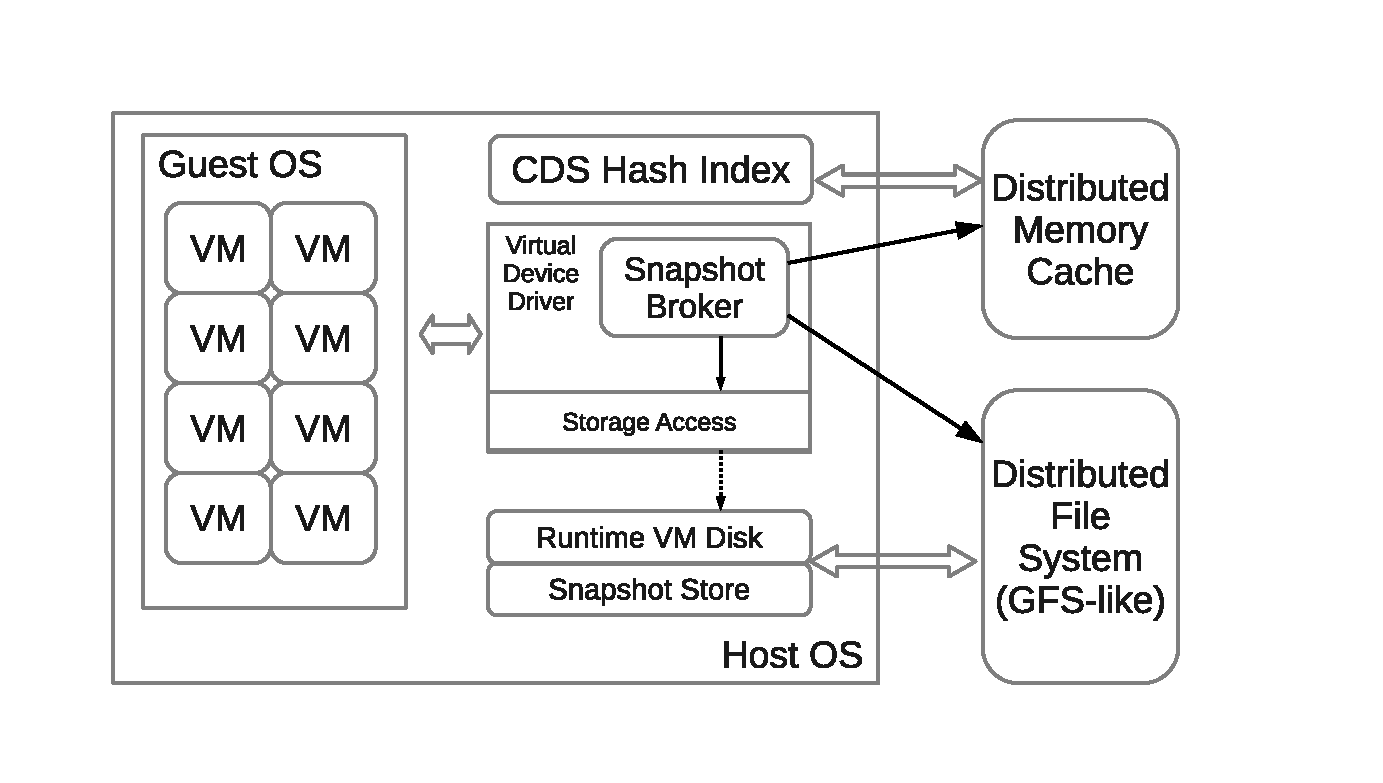
\epsfig{file=images/arch.eps, height=2in, width=2.66in}
  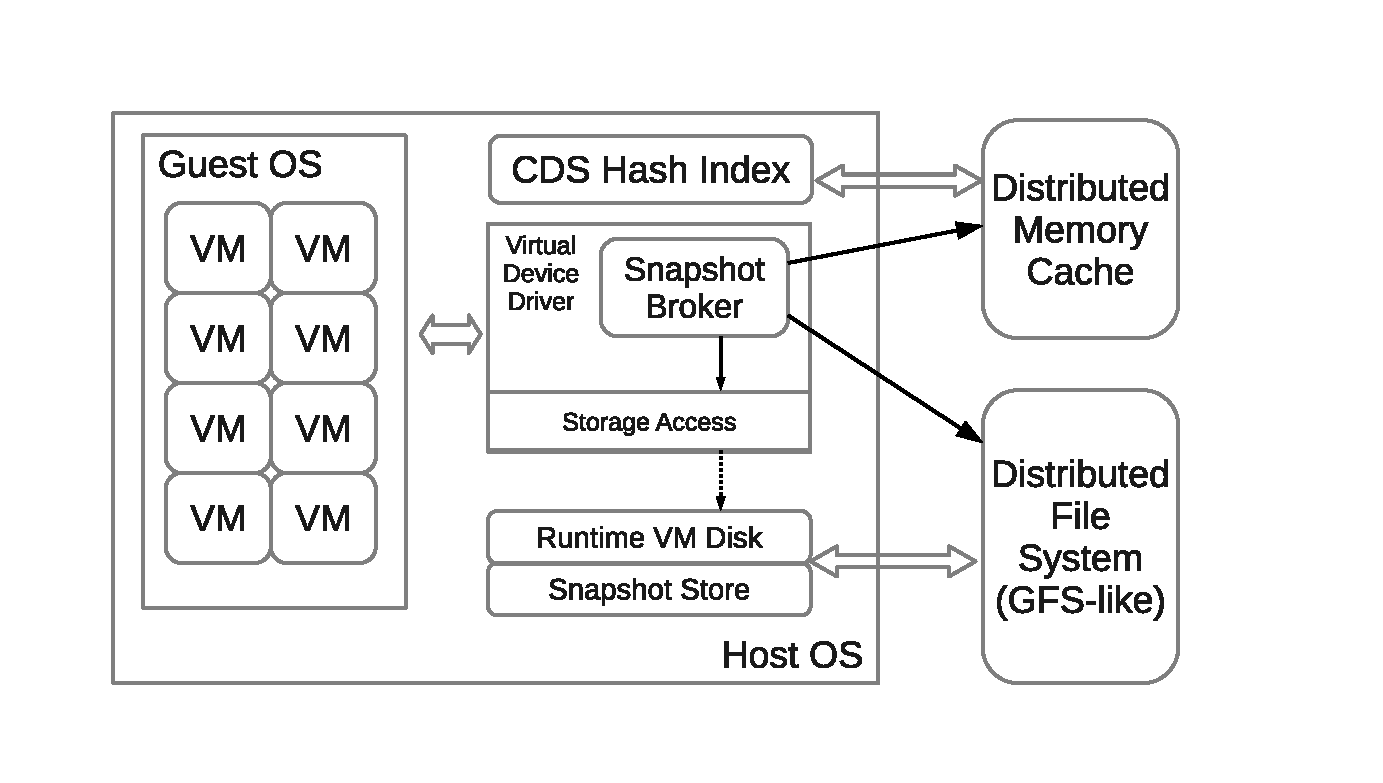
\epsfig{file=images/arch.eps, width=3.9in}
  \caption{Snapshot backup architecture of each node.}
  \label{fig:arch}
\end{figure}

The snapshot store 
supports data access operations such as \emph{get}, \emph{put} and \emph{delete}.
Other operations include data block traverse and resource usage report.
The snapshot data does not need to be
co-located with VM instances, and in fact they can even live in a different cluster to improve the 
data reliability: when one cluster is not available, we are still able to restore its VMs from another cluster which
holds its snapshot data. 
%to reduce the impact to our users.
%Get interface accepts a piece of data, write it to the underline data file, and return
%a reference to the caller. This reference then can be used in the put interface to
%retrive or delete the data, thus the caller of put interface must preserve the
%data reference for future use. 
%In addition to above standand data access operations, the snapshot service also supports
%\emph{scan} and \emph{quota} methods. Scan allows us to traverse all the data blocks of each VM
%in the snapshot store, and quota is used to acknowledge user how much space he
%has actually used.

Under the hood of snapshot store, it organizes and operates snapshot data 
in the distributed file system. We let each virtual disk has its own snapshot store, 
and no data is shared between
any two snapshot stores, thus achieve great fault isolation. For those selected popular data
that shared by many VM snapshot stores, we could easily increase its availability by having more replications.
%Since all the underline data structures is append only,
%upon a delete request, the corresponding data will only be marked rather than being deleted.
%A compaction will take place when deleted data has accumulated to a certain threshold, thus 
%reclaiming the disk space .




%The detail design and implementation of our distributed file system and various 
%storage subsystems would be too complicated to be intorduced here, and also beyond
%the scope of this paper. In the remaining section we will brief the model and interface of 
%our snapshot storage.

\subsection{Inner-VM Deduplication}
\label{sect:innerVM}

The first-level deduplication is logically localized within each VM.
%There are several reasons that we let each MS have  its own block store for localized duplication rather than sharing. 
%First, all data written to block store are already being processed by deduplication
%process, thus no sharing is necessary unless we want to perform additional deduplication
%inside the block store. Second, 
Such localization increases data independency between different  VM backups,
simplifies  snapshot  management and statistics collection during VM migration and termination,
and facilitates parallel execution of snapshot operations.
%Finally, this reduces the complexity of concurrent snapshot operations.

%\begin{figure}[htbp]
%  \centering
%  %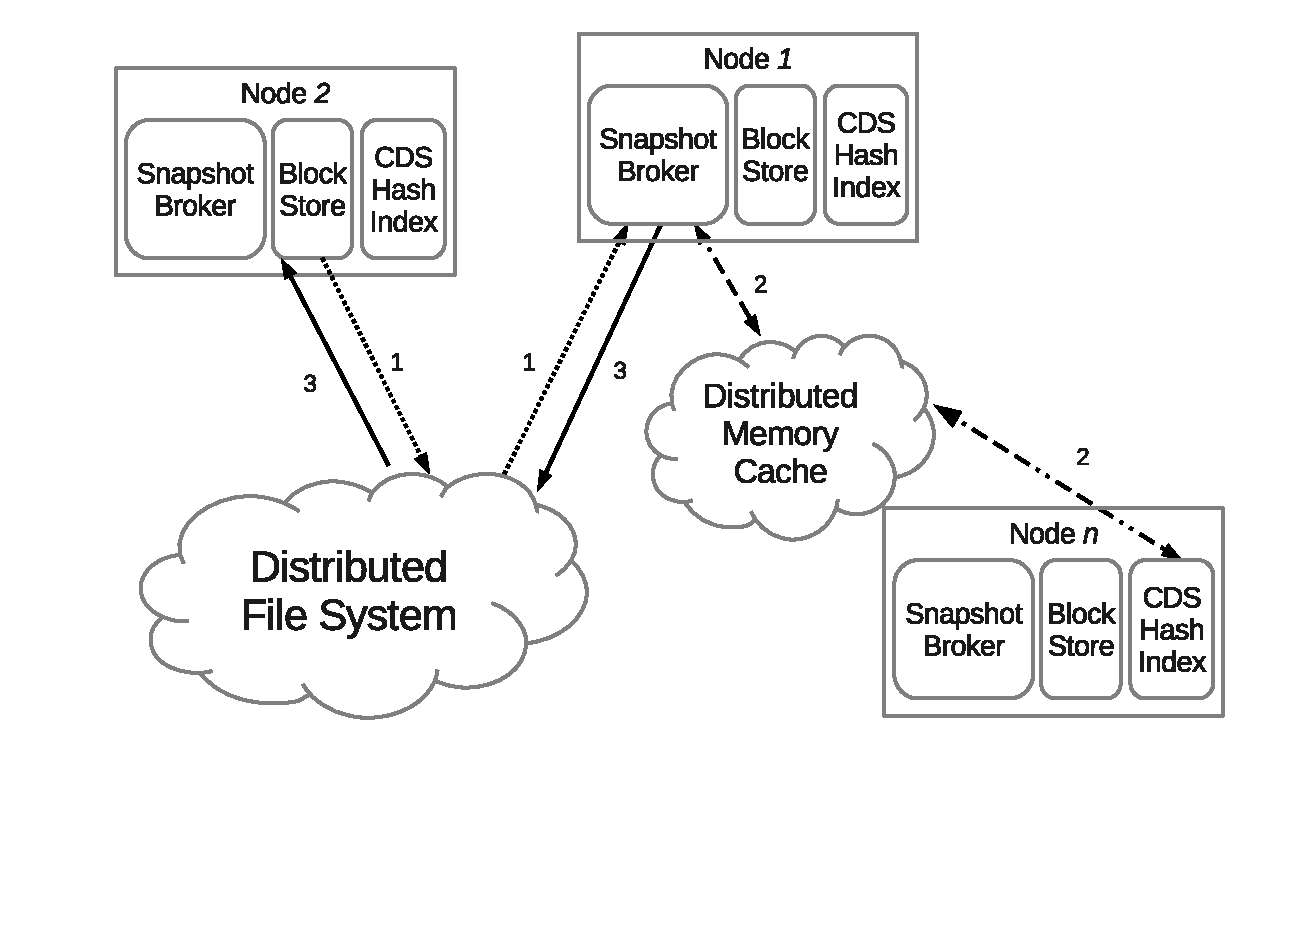
\epsfig{file=images/dedup_process.eps, height=2in, width=2.66in}
%  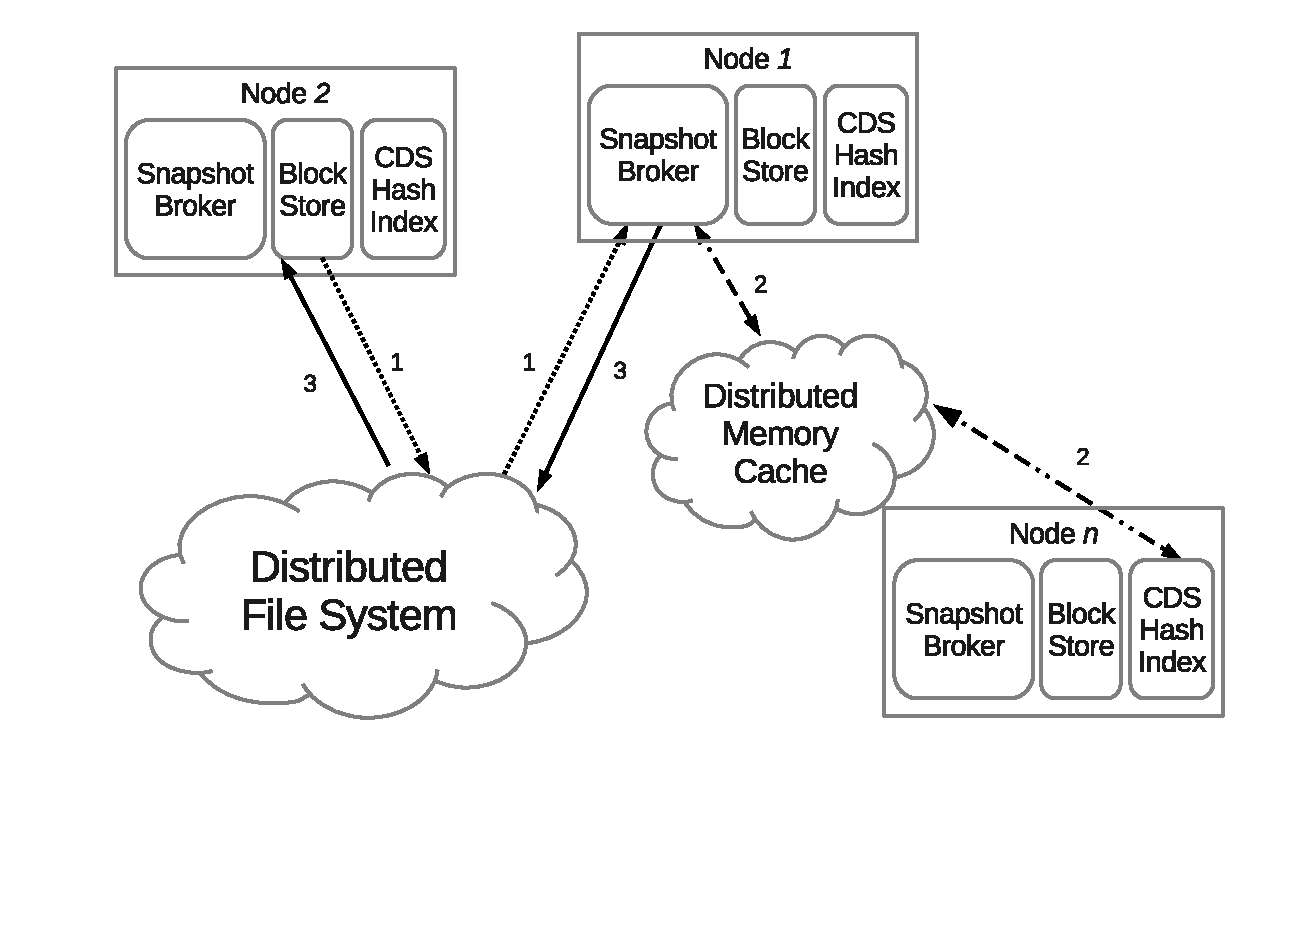
\epsfig{file=images/dedup_process.eps,  width=3.2in}
%  \caption{An example  of multi-level deduplication process.}
%  \label{fig:arch}
%\end{figure}
\begin{figure}[htbp]
  \centering
  %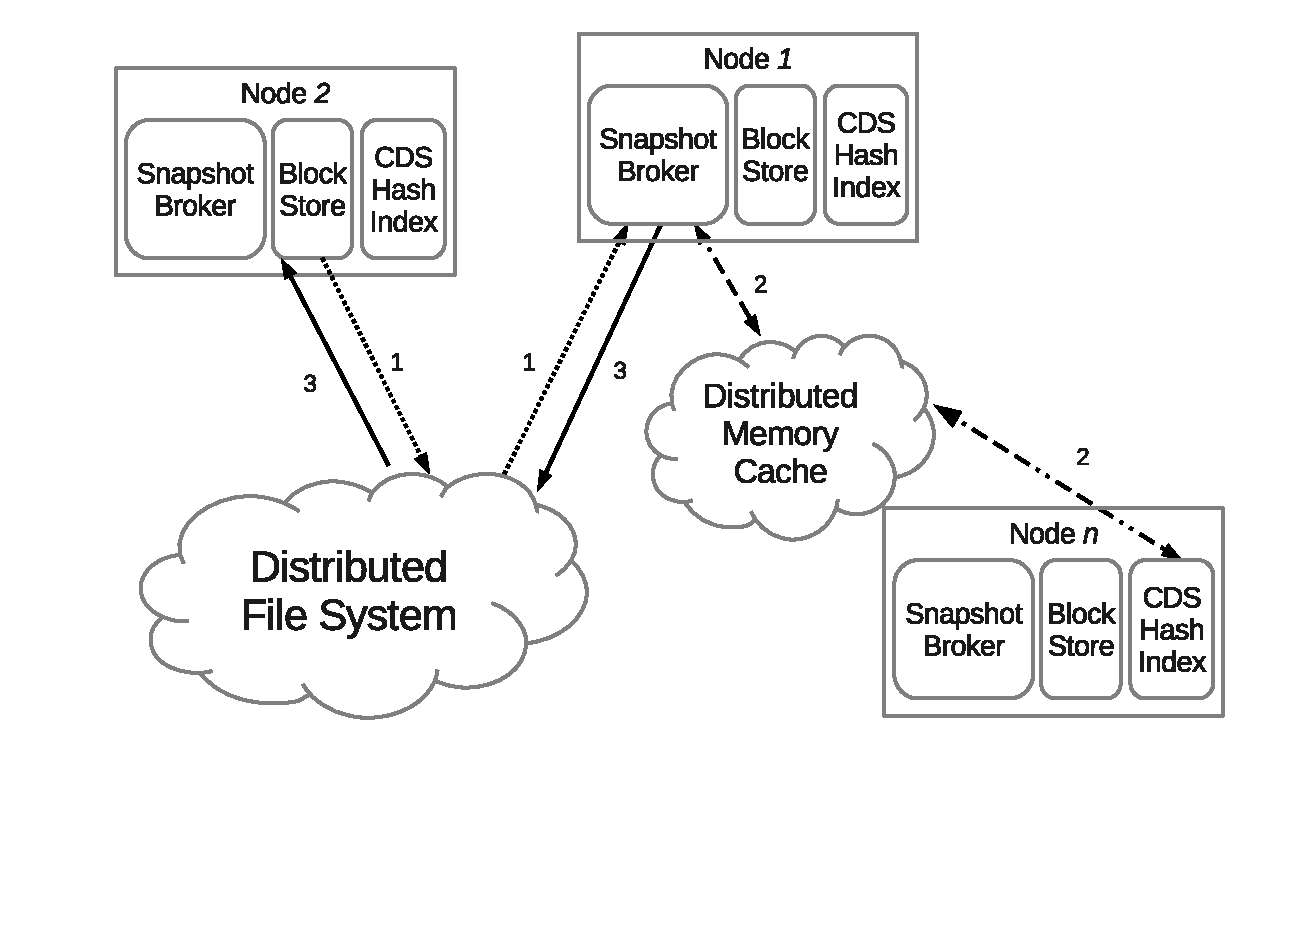
\epsfig{file=images/dedup_process.eps, height=2in, width=2.66in}
  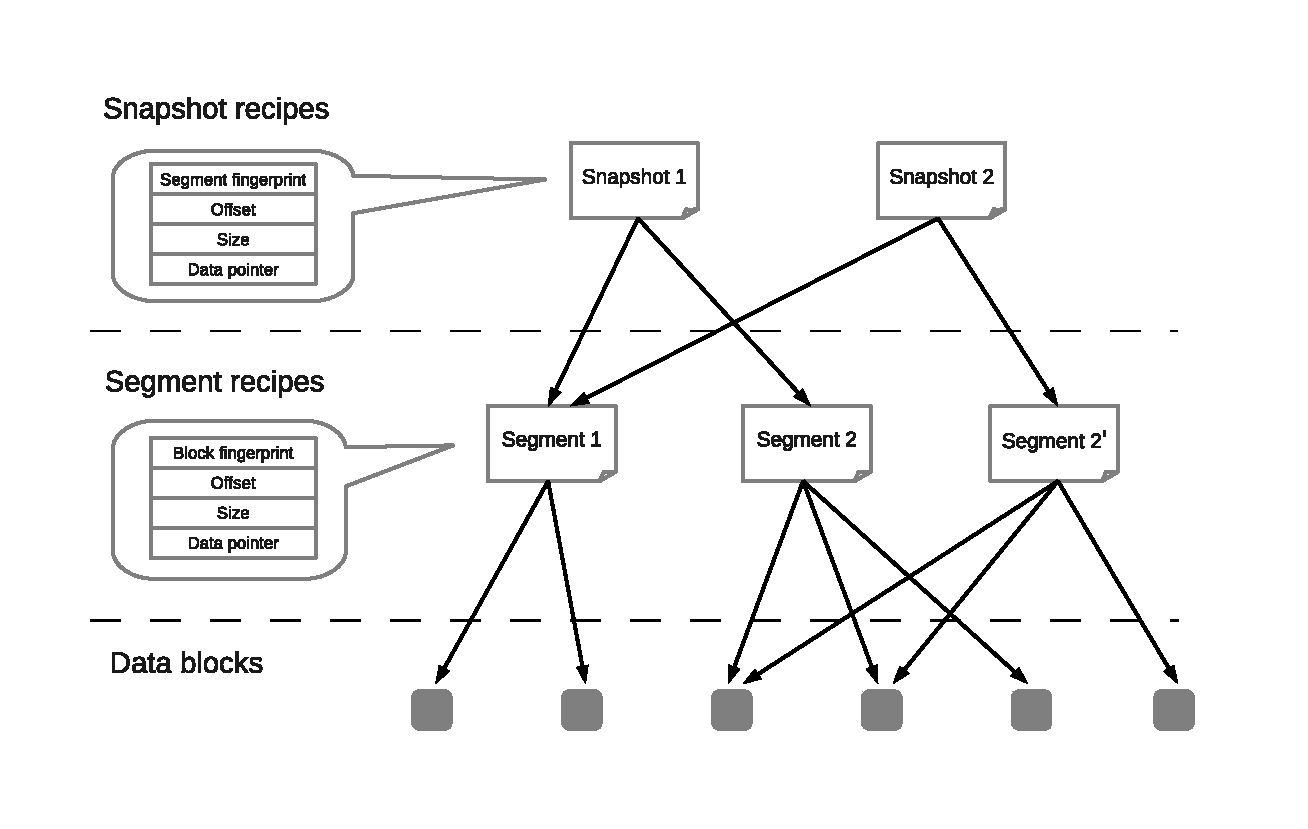
\epsfig{file=images/snapshot_representation.eps,  width=3.8in}
  \caption{An example of snapshot representation.}
  \label{fig:snapshot}
\end{figure}

The inner VM deduplication contains two levels of duplicate detection efforts and the representation of
each snapshot is correspondingly designed as a two-level level index data structure in the form of a hierarchical
directed acyclic graph as shown in Figure~\ref{fig:snapshot}.
An image file is divided into a set of segments and each  segment contains hundreds of content blocks from the bottom level.
These blocks are of variable-size, partitioned using
the standard chunking technique~\cite{similar94} with 4KB as the average block size. 
%To simplify the deduplication process, segments are aligned to fix-sized boundaries, currently using 2MB.
Segment metadata (called segment recipe) records its  content block hashes and data pointers. 
The snapshot recipe contains a list of segments and other meta data information.
\begin{itemize}
\item {\em Level 1 Segment modification  detection}.
If a segment is not changed, indicated by a dirty bit embedded in the virtual disk driver, its content blocks are not changed as well, thus its segment recipe can be simply reused. Operations at this level have almost no cost and most of unmodified data are filtered here. 

\item {\em Level 2  Block fingerprint comparison.}
If a segment is modified, we perform fine-grained deduplication using content blocks of this segment to compared with 
the same segment in
the previous snapshot (also called parent snapshot). Partial duplication
within the segment can be detected and eliminated. 
\end{itemize}

We choose this two-level structure because in practice we observe that during each backup period only a small amount
of VM data are added or modified. As the result, even the meat data of two snapshots can be highly similar,
thus aggregating a large number of content blocks as one segment can significantly
reduce the space cost of snapshot meta data. 
%Namely the  snapshort metadata starts with
%the representation of segment-level meta data. Each segment receipe can be further represented by
%a set of content block receipes.

How can we choose the length of a segment?
Instead of using variables-sized segments, we take a simple approach
to let every segment being aligned to the page boundary of each virtual image file.
For Aliyun, each VM image file is represented as a virtual disk file format
(called \emph{vhd} at Xen) and we use a dirty bit to capture if a page (or segment) of a virtual disk file 
has been modified or not to ease the segment-level deduplication.
%This is effective because  
%a vhd   file keeps the allocated inner blocks at the same positions until deletion,
%which means the locality of snapshot data is almost natively aligned. 
A dirty bit array is used to indicate which segments have been modified or not. 
Each page (segment) size in our implementation uses 2MB, which contains a large number of content blocks.
%Enforcing a boundary at every 2MB will 
%only break 0.2\% of total data blocks which is tiny.
% dirty bits array. This is because
%Inside the TapDisk driver, we maintain an array of \emph{dirty bits} to record the dirty area
%of runtime VM image file since the last snapshot, each bit represent a 2MB fix-sized
%data segment. During a snapshot operation, we only need to look at the dirty region
%rather than scan over the whold image file, which would be extremely slow.





%We let each virtual disk has its own block store rather than sharing for several reasons:
%first, all data written to block store are already being processed by deduplication
%process, thus no sharing is necessary unless we want to perform additional deduplication
%inside the block store. Second, such seperation will facilitate VM data stastics, 
%deletion and migration. Finally, this reduces the complexity of concurrent snapshot operations.

Once level-2 deduplication is activated for those segments that have been modified,
it requires memory to load  block fingerprints from the corresponding
parent snapshot's segment.
This scheme processes one segment at time and each segment of 2MB contains about 
500 content blocks on average given 4KB is the average block size.
That only takes a tiny amount of space to hold their fingerprints.
%Given  1-2 hours of window to backup snapshots and every VM has  on average about 40GB, there is enough
%time to search all segments sequentially~\cite{NOT-CLEAR-HERE}

\subsection{Cross-VM Deduplication with CDS}
\label{sect:crossVM}

The level-3 deduplication is to identify duplicated data blocks among multiple VMs through the index cache
of common data set (CDS).  CDS is the most popular content blocks 
among snapshots across all VMs. 
Each index entry contains  the block fingerprint and a reference pointer to the location of its real content
in the snapshot content block store.
%The structure of CDS meta is not different from the segment recipe we discussed above, 
%except that it is partitioned into many small slices so that each node is easy to load its own slice. 

At the runtime, the CDS index resides in a distributed  memory lookup table  
implemented using Memcached~\cite{memcached} to leverage the aggregated memory in a cluster.
Th usage of memory at each machine is small and thus  this scheme  does not
lead to  a memory resource contention with the existing cloud services.
%For example, in our current implementation setting at Aliyun, we use up to  150MB memory per node during night backup
%including CDS and other metadata for all levels of deduplication. Most of memory resource (48GB per node 
%in our experiment) is used for existing  applications.
CDS raw data stored  in the distributed file system
has multiple copies in different machines for the purpose of fault tolerance and 
while providing high read throughput.  
%The data of CDS is stored in a special block store in the distribued file system.

% which doesn't belong to any VM disk.

%CDS meta assignment is done statically, each slice of CDS meta has one primary and two backup nodes.
%During the system bootup, snapshot storage controller will read the assignment, 
%load its primary portion of CDS meta from distributed file system. Loading the backup portion
%of CDS is due upon a query arrives for it. Everyday the CDS assignment and CDS data will be checked
% for updates and reloaded if necessary.

%Behind the scene there is a offline map-reduce job, which will periodically scan the block stores
%in the entire cluster and perform a ``word counting''. High frequency blocks are then added to the CDS if its count 
% is greater than threshold, which is pre-defined by the system memory restrictions.
To control the size of searchable common data in this global setting, we focus on those items that 
are most popular based on the historical snapshot data and the popular analysis is conducted periodically to ensure 
meta data freshness to match the latest data access trend.
There are two advantages to exploit this.
First, a smaller CDS reduces overall resource requirement while covering most of data duplication.
Second, knowing this small set of data is shared heavily makes the fault tolerance management 
easier because we can replicate more copies to mitigate the failure.

In Aliyun's VM cloud, each VM explicitly maintains  one OS disk, plus one or more data disks.
During VM's creation, its OS disk is directly copied from user's chosen base image.
Given the separation of OS disks and data disks, we study  their characteristics separately.
We expect that data related to OS and popular software installations are not frequently
modified or deleted, to facilitate analysis we call them \emph{OS-related} data, 
and the rest of data, either from OS or data disks, are called \emph{user-related} data.
%base image data as a hint.Through users may change configurations, install software, or write user data into OS disk,
%Thus most of content blocks for the OS related snapshots  shall keep unchanged.
%This is verified in  Section~\ref{sect:exper}.
We have studied the popularity of common blocks in the OS and data disks from a dataset
containing over 1,000 VMs, taking their first snapshots to watch the cross-VM duplication pattern 
(scale of OS disk sampling is smaller due to performance impact to user VMs).
Figure \ref{fig:zipf-data} shows the duplicate count for unique data blocks sorted by their ranking in 
terms of the duplication count. $Y$ axis is the popularity of a data block in a log scale 
measured its duplicate count among snapshots. $X$ axis is the identification of data blocks in a log scale
sorted by their duplicate rank.  The rank number 1 is the block with the highest number of duplicates.
These two curves exhibit that the popularity of common blocks partially follows a Zipf-like distribution.
%$Y$ axis is the popularity of an OS block in a log scale 
%measured its duplicate count among snapshots. $X$ axis is the identification of OS blocks in a log scale
%sorted by their duplicate rank.  
%For the top ranked blocks, there is a flat line in terms of duplicate counts. That
%is because there are a large number of OS blocks which have appeared in all copies of such OS releases.


\begin{figure}[htbp]
\centering
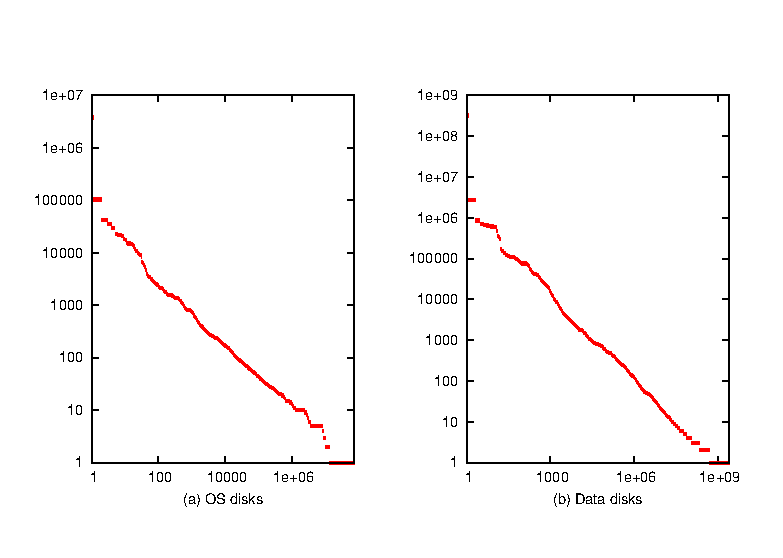
\epsfig{file=images/vector.eps, width=3.8in}
%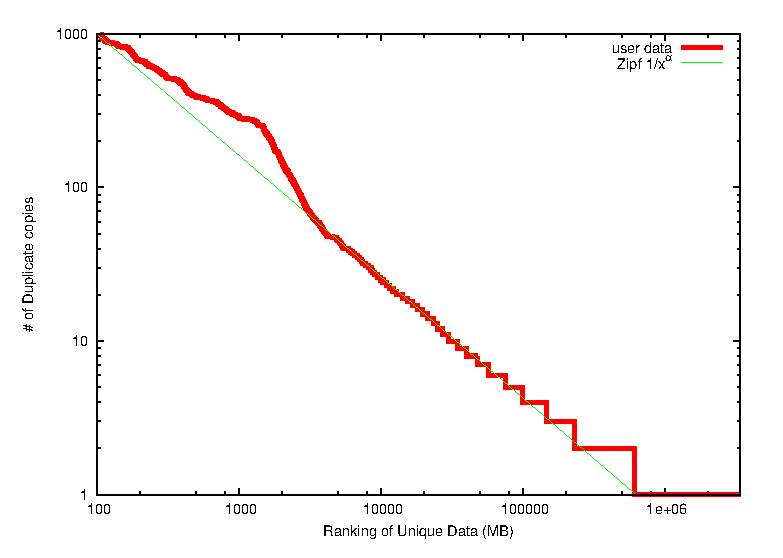
\epsfig{file=images/log-log.disk.eps, width=3in}

%\begin{tabular}{cc}
%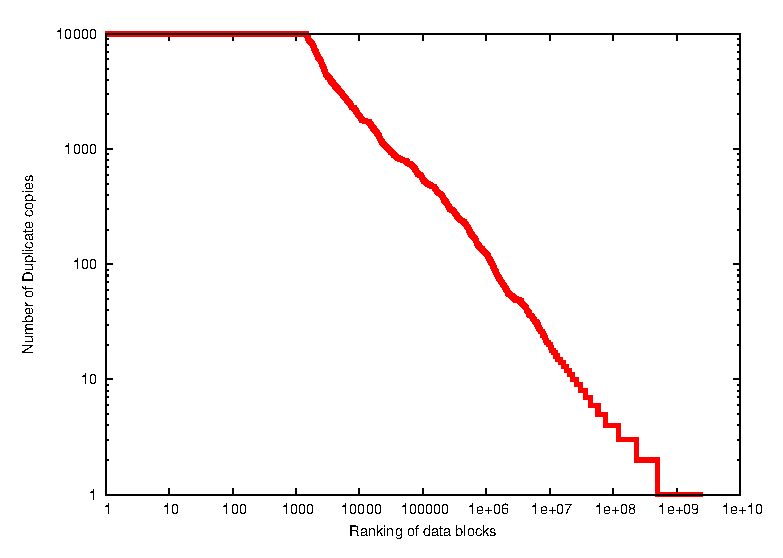
\epsfig{file=images/datadisk.count_rank.eps, width=1.5in} &
%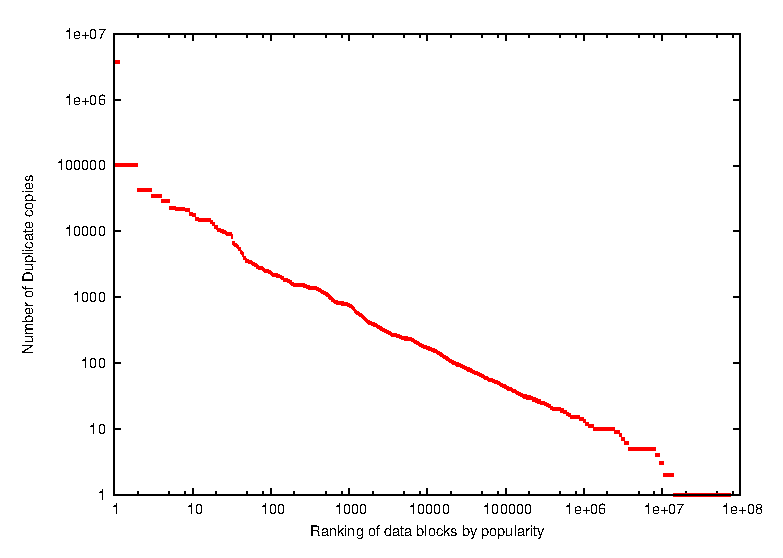
\epsfig{file=images/35vmos.count-rank.eps,width=1.5in}
%\end{tabular}

\caption{Number of duplicates vesus ranking}
\label{fig:zipf-data}
\end{figure}

%\begin{figure}
%\centering
%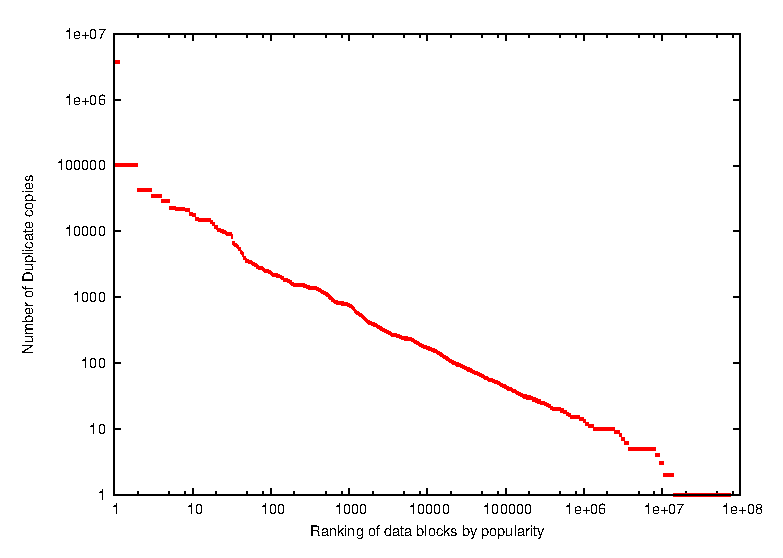
\epsfig{file=images/35vmos.count-rank.eps,width=3in}
%\caption{ Duplicate count of  common OS blocks in a log scale.}
%\label{fig:OSpopular}
%\end{figure}

Base on the Zipf-like distribution pattern, many previous analysis and result on web caching may apply.
In general this indicates a small set of popular data dominates data duplication.
Although we already know OS-related data are heavily duplicated among OS disks, 
it still surprises us that user-related data follow a similar pattern.
Therefore, we collect the CDS by performing global reference counting through map-reduce for all
blocks in snapshot store, and select the most popular ones base on the memory limitation of
CDS hash index. 

The CDS collected from user-related data is generally proportional to the data size.
As discussed in Section~\ref{sect:exper}, selecting about 1\% of data (after level 1 and level 2 deduplication)
can cover about 38\% of data blocks. Consider we allow maximum 25 VMs per machine, each VM has
about 30GB of user-related data, having 10 snapshots in its snapshot store and the data change ratio during
each backup is 10\%, this translates to 15GB CDS data per machine, and the 
memory cost by CDS hash index is about 150MB per machine.
On the other hand, the CDS from OS-related data is only relvant to the number of OS releases.
Our experiment on 7 major OS releases shows that about 100GB of data is never modified, and we expect
it won't grow over 200GB in the near future. So it would cost the entire cluster 2GB of memory to
store its hash index, or 20MB per machine on a 100 node cluster. On average each OS disk has about 10GB
of data that can be completely eliminated in this way.
\comments{
As the number of VMs increases, the popularity of common blocks for data disks changes.
But this increase has a small impact on OS block popularity because 
there are a limited number of OS releases used by VMs. We let CDS cover the common OS blocks first and
our CDS selection strategy is designed as follows. 

\begin{itemize}
\item First, most popular items from OS disks are selected as the initial CDS.
Our experiment data shows that about 
100GB data from 7 most popular OS releases
can at least cover over 70\% of OS snapshots and the index of these 100GB OS blocks
only takes about total 1GB in the CDS index and then memory requirement per node 
for duplicate search a large cluster is tiny.
We expect that the OS CDS index may grow up to 2GB in order to cover large varieties  of commonly deployed
OS releases in practice.
\item Second, the degree of duplication is computed for the rest of blocks in snapshot store, and
% and also snapshot 
%blocks of user data items stored in the OS disk (some users store data in their OS disks).
the  most popular items are selected. As discussed in Section~\ref{sect:exper}, 
that about 1\% of data blocks are selected based on their duplicate counts and these popular blocks
can cover about 38\% of data  blocks appeared in various snapshots after level 1 and level deduplication.  
The memory size per node used for CDS is within 150MB.
\end{itemize}}
Thus in total the CDS index size per node takes less than 170MB in a large cluster bigger than 100 nodes, 
covering over 47\% of blocks in OS and data disks after inner-VM deduplication.
This memory usage is well below the limit required by our VM services.

\subsection{Illustration  of multi-level deduplication process}


\comments{
\begin{figure*}
  \centering
  %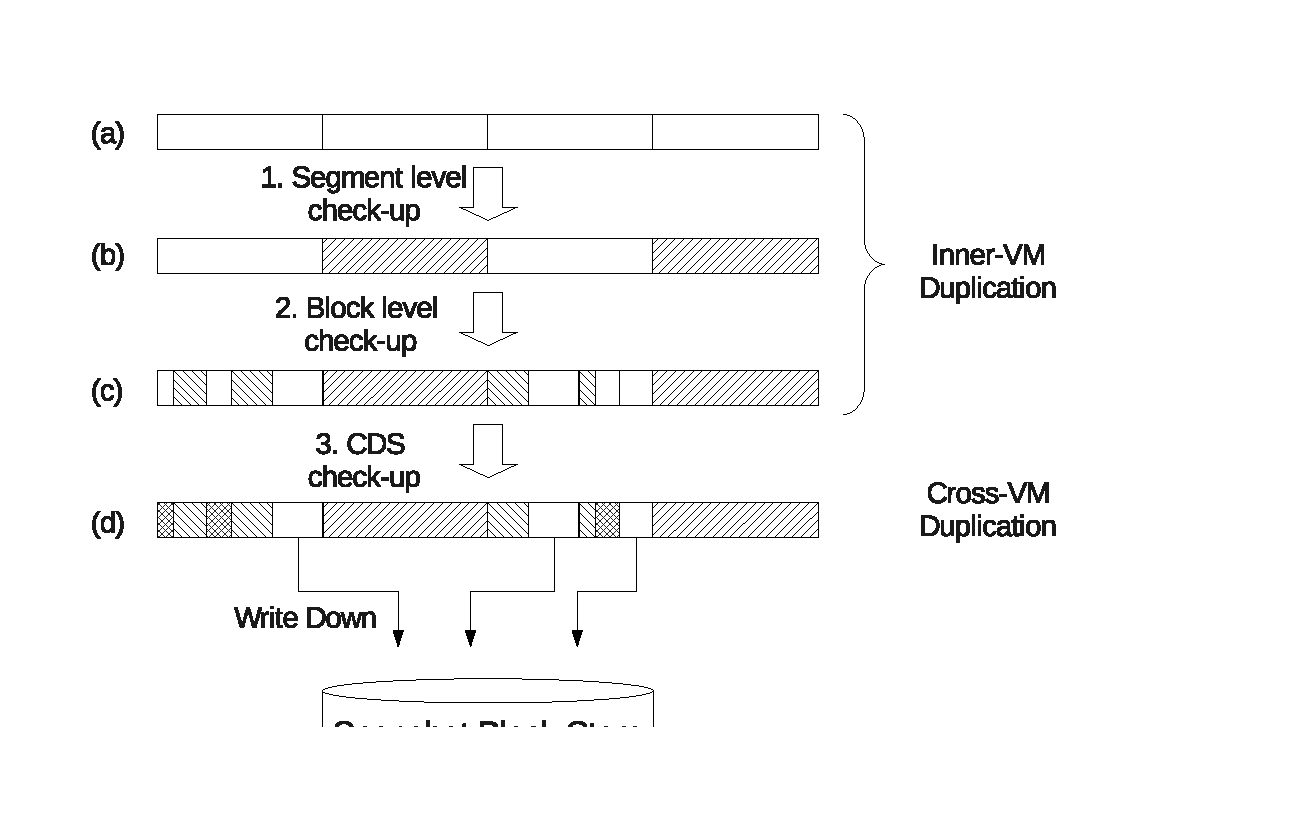
\epsfig{file=images/dedup_flow1.eps, height=2in, width=3.5in}
  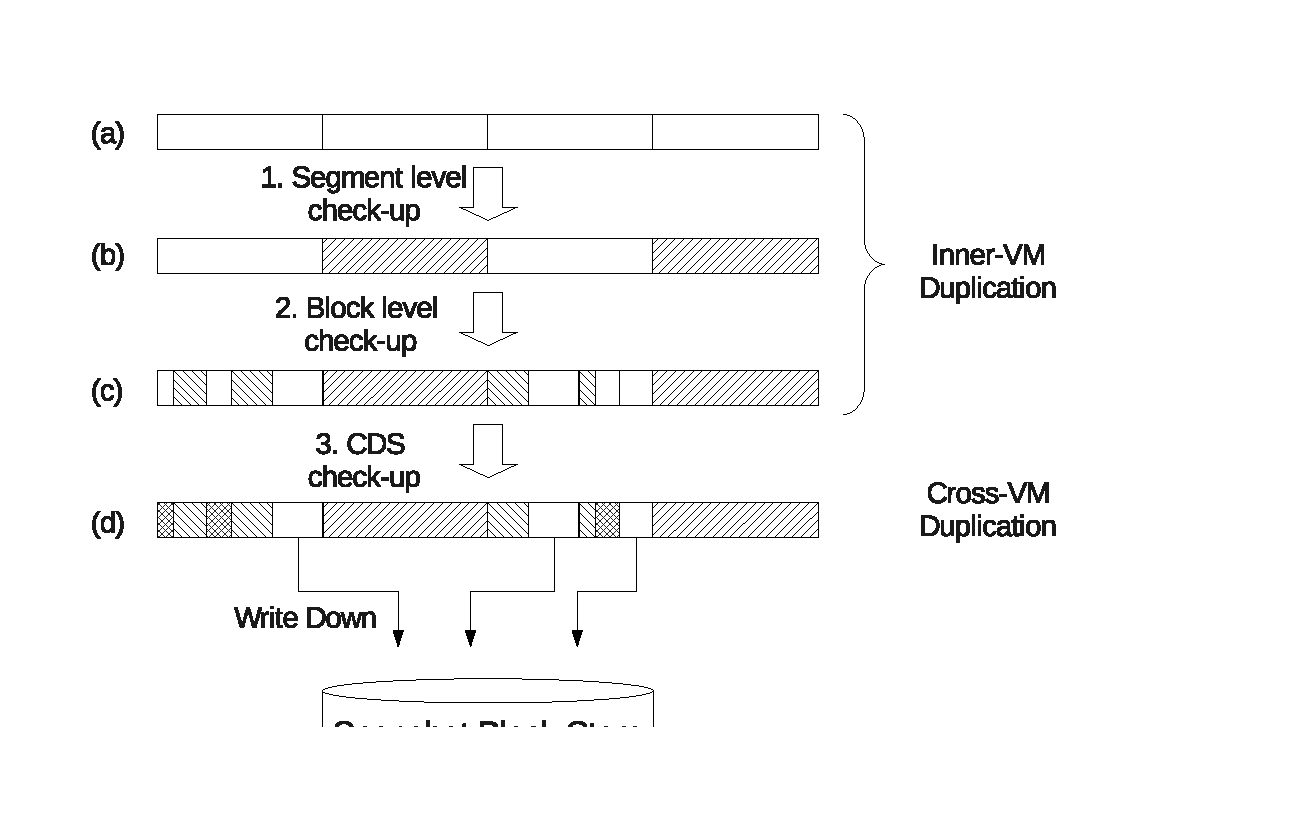
\epsfig{file=images/dedup_flow1.eps,  width=6in}
  \caption{Flow of deduplication.}
  \label{fig:tapdisk}
\end{figure*}
 

The 3-level deduplication process can be summarized as four steps:
\begin{list}{Dedup}{}
\item {Dirty bits: Copy the unchanged portion of snapshot recipe from parent snapshot, base on dirty bits.}
\item {Locality: Divide dirty segments into blocks, compare to the corresponding segment recipe at the same position of parent snapshot, if duplicate, copy the data reference into segment recipe.}
\item {CDS: Check if this data exist in the CDS, if yes, copy the returned data reference. Otherwise, write data block to block store, save the returned reference into segment recipe.}
\item {Save meta: write down the segment recipes and snapshot recipe when finish.}
\end{list}

}


%%Our deduplication process is divided into three levels, at each level, we eliminate the most of duplicate data with available knowledge, preventing them from going further because deduplication at deeper level is more expensive.
%
\begin{figure}
  \centering
  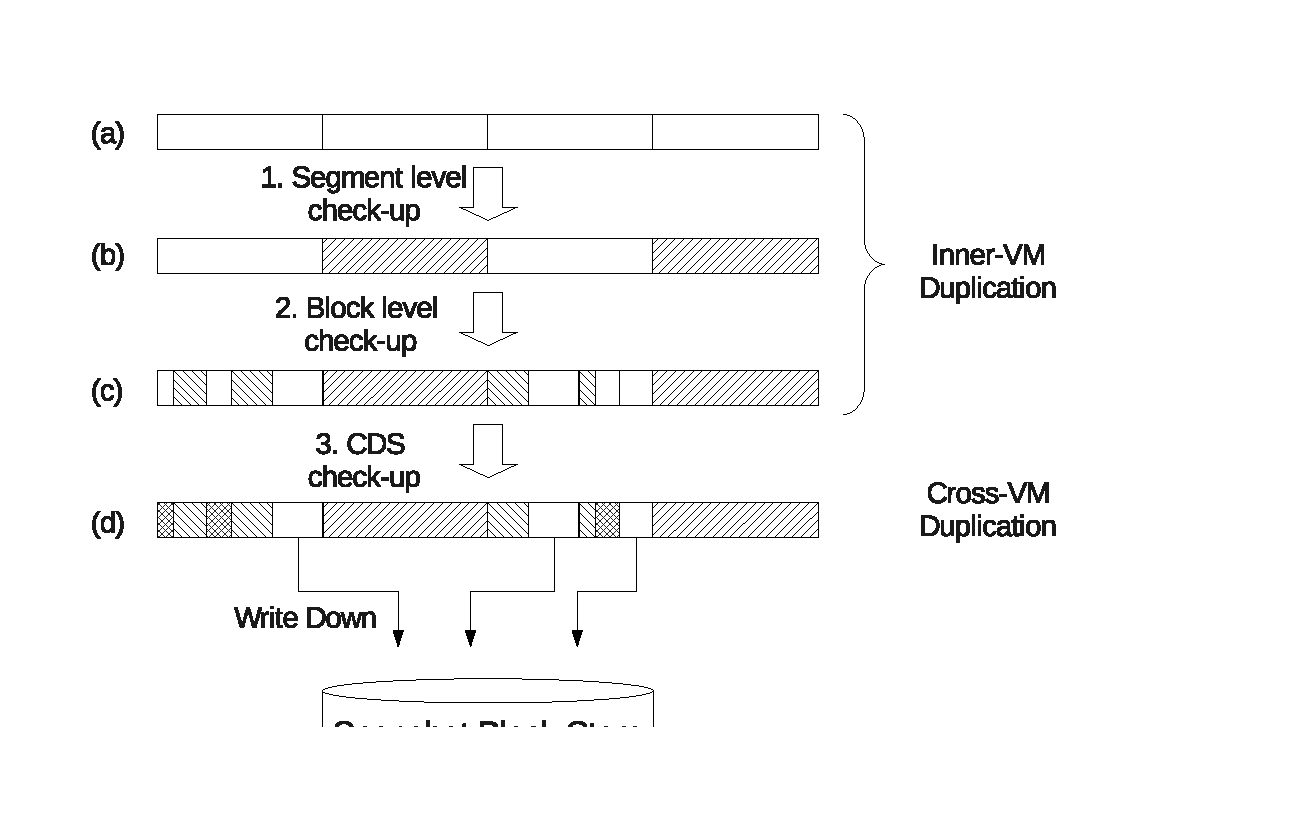
\epsfig{file=images/dedup_flow1.eps, width=3.8in}
  \caption{Illustration of snapshot deduplication dataflow.}
  \label{fig:dedupflow}
\end{figure}

We illustrate the steps of 3-level deduplication in Figure~\ref{fig:dedupflow}, which can be summarized as 5 steps:
\begin{enumerate}
\item {\em Segment level checkup.}
As shown in Figure~\ref{fig:dedupflow} (a),
when  a snapshot of a plain virtual disk file is being created, we first check the dirty bitmap 
to see which segments are modified. If a segment is not modified since last snapshot, 
it's data pointer in the recipe of the  parent snapshot  can be directly copied into 
current snapshot recipe (shown as the shadow area in Figure~\ref{fig:dedupflow} (b)).

\item {\em Block level checkup.}
As shown in Figure~\ref{fig:dedupflow} (b),
for each dirty segment, we divide it into variable-sized blocks,
and compare their signatures with  the corresponding segment recipe in the previous snapshot (called parent
snapshot). 
For any duplicated block, we copy the data pointer directly from the parent segment recipe. 
\item {\em CDS checkup.} For the remaining  content blocks whose duplicate status is unknown,
Figure~\ref{fig:dedupflow} (d)
shows  a further check to compare  them with  the cached signatures in the CDS by querying
the CDS hash index. If there is a match, the corresponding data pointer from the CDS index is
copied into the segment recipe. 
\item {\em Write new snapshot blocks :}
If a data block cannot be found in the CDS index, this block is considered to be a new block
and such a block is to be saved in the snapshot store, the returned data pointer is
saved in the  segment recipe.
\item {\em Save recipes.} Finally the  segment recipes are saved in the  snapshot block store also.
 After all segment recipes are saved, the snapshot recipe is complete and can be saved.
\end{enumerate}

If there is no parent snapshot available, which happens when a VM creates its first snapshot, 
only CDS-based checkup will be conducted. 
Most of the cross-VM duplication, such as OS-related data, is eliminated
at this stage. 
%Later snapshot will very likely find these data are not changed and simply copy the data pointers from parent snapshot.
%This is important because most of the cross-VM duplication, such as OS related data and popular software data, is eliminated
%at this stage. Later snapshot will very likely find these data are not changed and simply copy the data pointers from parent snapshot.
 %, design considerations, architecture

\section{Evaluation}
\label{sect:exper}

We have implemented a snapshot deduplication scheme on the Aliyun's cloud platform.
Our experimental evaluation has the following two objectives:
1) Analyze the commonality of content data blocks and the popularity  of hot items. We 
examine the impacts of CDS size on deduplication ratio.
2) Assess the effectiveness  of 3-level deduplication for reducing the storage requirement of snapshot 
backup. 

\subsection{Experimental setup}

An Aliyun cluster we target is over 1000 nodes with 16 cores and 48GB memory
and each node hosts 25 VMs.
We are running our deduplication/backup  service on 100 nodes.
Memory usage is about 150MB space per node during backup and
the CPU usage is very small during the experiments. 
Based on the data studied,  each VM has about  40GB of storage  data usage on average
and each of OS disk and data disk takes about 50\% of storage space.
The backup of VM snapshots is completed within two hours  every day,
and that translates to a backup throughput of 139GB per second, or 500TB per hour.
For each VM, the system keeps  10 automatically-backed snapshots in the storage while
a user may instruct extra snapshots to be saved.

% the system must finish saving daily snapshots of all VMs in 2 hours. In our typical 1000 nodes cluster, each node hosts 25 VMs, each VM has 40GB of data on average, that translates to backup throughput of 139GB/second, or 500TB/hour.

%In our snapshot deduplication architecture, CDS is the key to achieve greater deduplication than
%incremental backup solutions. Our basic assumption of CDS us that VM disks, especially OS disks,
%have huge amount of data in common, and such common data can be represented by a relatively smaller data set
%because of their high appearence frequency. As a result, the major portion of snapshot deduplication effect shall 
%emerge from eliminating the duplication of such a small data set. In this section, we evaluate
%the effectiveness of CDS using real user VM disks from our production VM cluster.

We have used a storage dataset of  1323 VM users collected from 100 Aliyun's cloud nodes  to evaluate the effectiveness.
In this dataset, there are 10 snapshots per each VM user and the total amount of space investigated 
is 23.5 terabytes.
Each VM file is  divided into a set of content blocks using
TTTD chunking~\cite{??} with an average size of 4KB. Each segment is of size 2MB.  
Popularity is computed by using 90\% of dataset, which reflects our setting that the system recomputes
CDS every 1-2 days to catch up the popularity trend.

%seg, and we performed global perfect deduplication 
%to caculate the number of duplicate copies of each individual unique block. We choose 2KB, 4KB, 16KB as the minimum, average
%and maximum block size
The signature for variable-sized blocks is computed using  their SHA-1 hash. 
%OS data
%user data: zipf
%prediction
%say something about aliyun


%To compare the effectiveness with a full deduplication approach with an approximation,
%we use  extreme binning and perfect deduplication~\cite{extreme_binning09}. 
%For perfect deduplication and extreme binning, each snapshot is also divided into chunk blocks
%using TTTD with an average size of 4KB. The original extreme binning work uses the whole file
%as the input unit and  this size is too big in our system. 
%Thus we split each image snapshot file into variable-sized segments base on the block hash list, 
%using TTTD with average size of 2MB.

\subsection{Effectiveness of 3-level Deduplication}

\begin{figure}
  \centering
  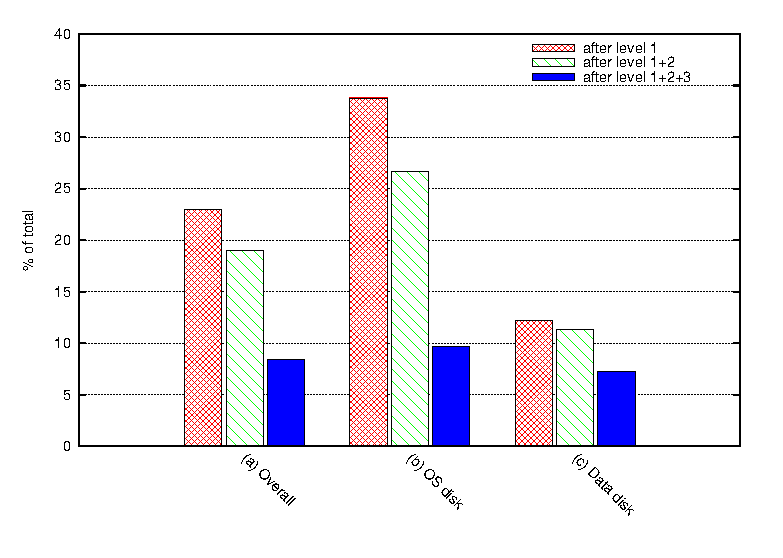
\epsfig{file=images/overall_effect.eps, width=3in}
  \caption{Impacts of 3-level deduplication. The height of each bar is the data size after 
deduplication divided by the original data size and the unit is percentage. }

  \label{fig:overall}
\end{figure}

Figure~\ref{fig:overall} shows the overall impact of 3-level deduplication.
The X axis shows the overall impact in (a),  impact on OS disk in (b), and impact on data disk in (c).
Each bar in the Y axis shows the data size after deduplication divided by the original data size.
Level-1 elimination can reduce the data size to 22\% of original data, namely it delivers close 80\% reduction.
Level-2 elimination applied after level 1
reduces the size further to 16\% of original size, namely it delivers additional 6\% reduction.
Level-3 elimination together with level 1 and 2
reduces the size further to 9\% of original size, namely it delivers additional 7\% reduction.
Level 2 elimination is more visible in OS disk than data disk, because data change frequency is really small
when we sample last 10 snapshots of each user in 10 days. Nevertheless, the average impact of level 2 is also significant.
A 6-7\% of reduction from the original data represents about 600-700TB of space.


\begin{figure}
  \centering
 %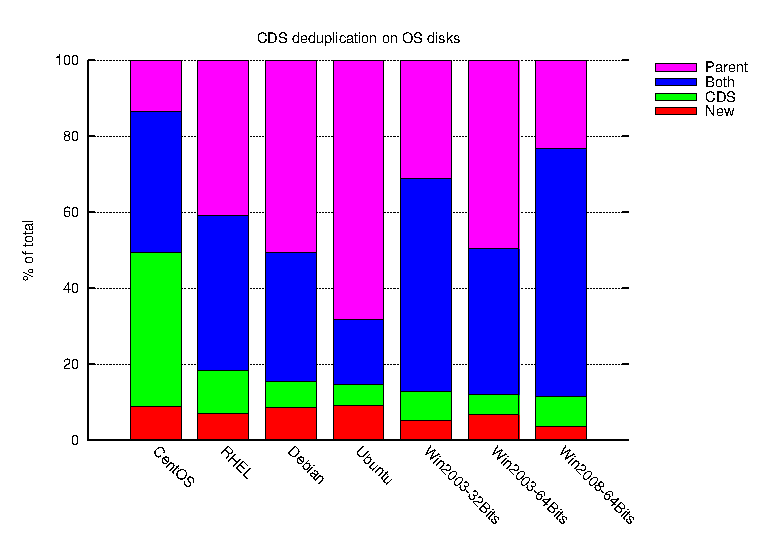
\epsfig{file=images/os_cds_sim.eps, width=3in}
  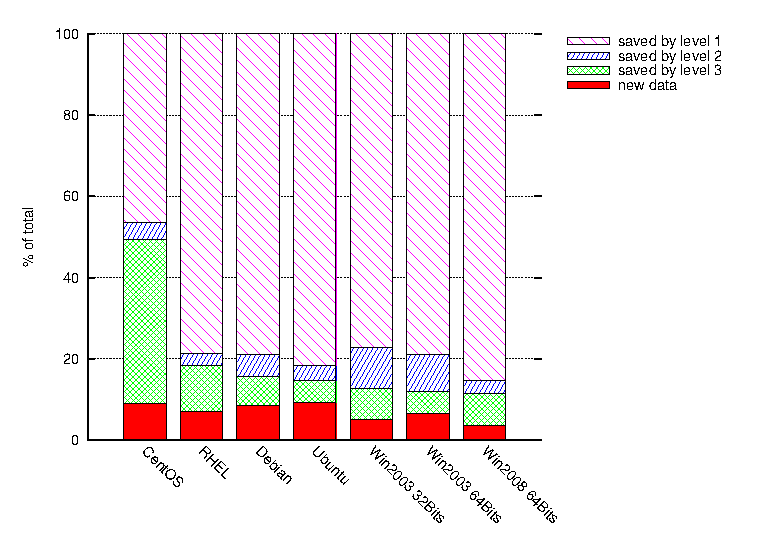
\epsfig{file=images/3level_os.eps, width=3in}
  \caption{Impact of 3-level deduplication for OS releases.}
  \label{fig:oscds}
\end{figure}

To see the impact of multi-level deduplication on different OS releases, we choose 7 major OSes in Aliyun's
VM cloud platform and they are: 
Win2008 Server 64 bits, Win2003 Server 32 bits, Win2003 Server 64 bits, RHEL, CentOS, Ubuntu Server and Debian (all Linux
distributions are 64 bits).
Then we examine 5 VM user disks from each OS, and 10 snapshots for each VM. These VMs have been actively used by their
owners. 
%Some of  OS disks are modified frequently and in some cases,  users even store a large amount of user data on
Figure~\ref{fig:oscds} shows the impact of different levels of deduplication for different OS releases.
In this experiment, we tag each block as  ``new''
if this block cannot be deduplicated by our scheme and thus has to be written to the snapshot block store;
``CDS''  if this block can be found  in CDS;
``Parent segment'' if  this block is marked unchanged in parent's segment recipe.
``Parent block'' if  this block is marked unchanged in parent's block recipe.
With this tagging, we compute the percentage of duplication accomplished by level-1 inner VM deduplication,
level-2 inner VM deduplication and level 3 cross-VM deduplication.
As we can see from Figure~\ref{fig:oscds}, level-1 deduplication accomplishes a large percentage of elimination
this is because the time interval between two snapshots in our dataset
is quite short and the Aliyun cloud service makes a snapshot  everyday  for each VM.
On the other hand,  CDS still finds lots of duplicates that inner VM deduplication can't find,
contributing about about 10\% of reduction on average.

%Combining OS disks in all the VMs, we see the overall 7.4TB of data is reduced to 512GB. 
%The extreme binning approach can reduce this data set to 542GB, which is slightly worse. As a reference, 
%perfect deduplication achieves 364GB in this experiment.

Overall speaking, inner   VM deduplication or  CDS-based deduplication
can work well alone, but by combining them together we get a fairly good and stable deduplication ratio to 
all kind of OSes. 
Compared to a traditional dirty bit approach based on pages of
each file (e.g. segment in our scheme),
our CDS-based level 3 approach  can save additional 50\% storage space because many of level 2 block
content can be eliminated using the CDS also.

\subsection{Coverage of common data blocks}

%We study characteristics of common data blocks among snapshots of VM users
%and examine the impacts if we only store a relative small amount of common data blocks to be sored in the CDS server.
%There are two advantages to exploit this.
%First, a smaller CDS reduces overall resource requirement while covering  most of data blocks in snapshots.
%Second a smaller CDS makes the fault tolerance management  easier because we can replicate  more copies
%to mitigate the failure.

%We consider each virtual disk contains two parts: OS partition and regular user data partition
%and study their characteristics seperately.
%In Aliyun's VM cloud, each VM explicitly maintains  one OS disk, plus  one or more data disks.
%During VM's creation, its OS disk is directly copied from user's choosen base image.
%Since  they dare brought by the operating system and popular 
%software installations,  they are rarely modified or deleted.
%base image data as a hint.
%Through users may change configurations, install software, or write user data into OS disk,
%but most of the OS related data shall keep unchanged. 

%Previous study has also supported this\cite{vmimage}. Therefore, we can let all OS disks share these
%common data in their snapshot backups.
%We choose user's data disks rather than OS disks in thie experiment for several reasons: First, the data in OS disks are 
%instinctively highly similar, because most of the VM users only make some common or unique but tiny changes to their OSes,
%so the data duplication pattern in OS disks cannot reflect the real distribution of general user data.
%Second, the data disks are way more important in terms of data safty and backup because they are 
%what users really care about.

%Furthermore, our study on user's data disks has shown that the duplication pattern of
%variable-sized data blocks follows \emph{Zipf-like} distribution. As a result, the major portion of 
%deduplication effect will emerge from eliminating the duplication of frequently seen data.
%define CDS


\comments{
\begin{figure}[htbp]
\centering
%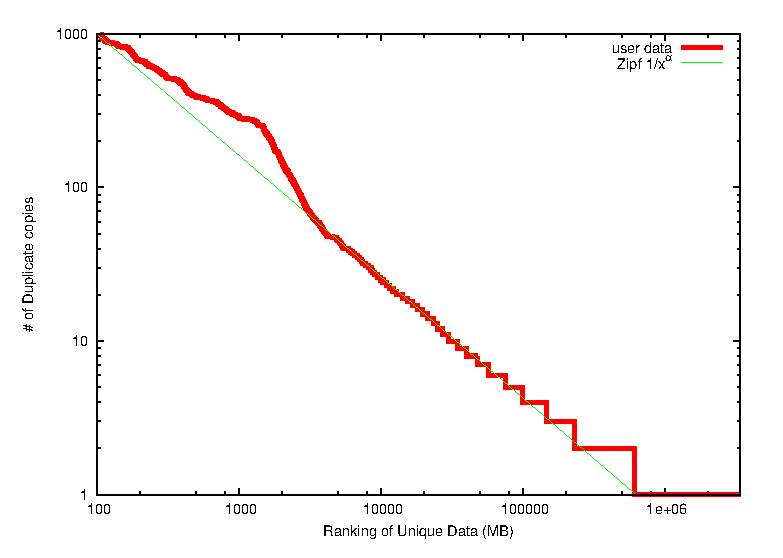
\epsfig{file=images/log-log.disk.eps, height=2in, width=2.66in}
%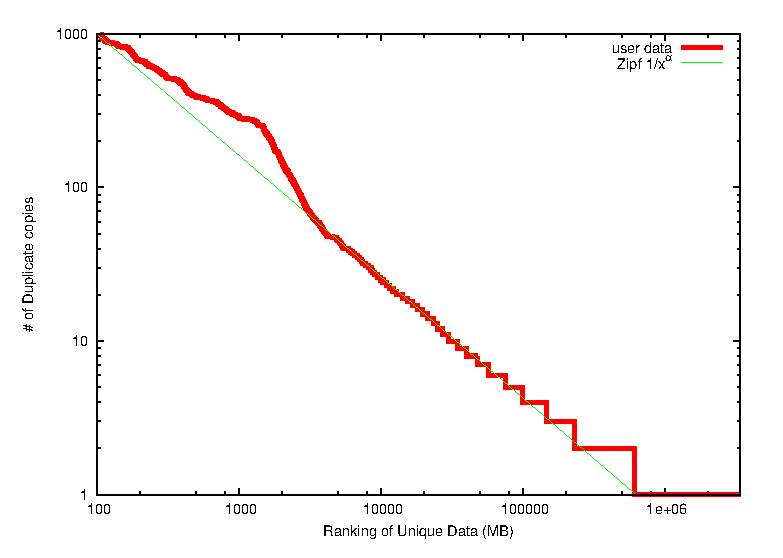
\epsfig{file=images/log-log.disk.eps, width=3in}
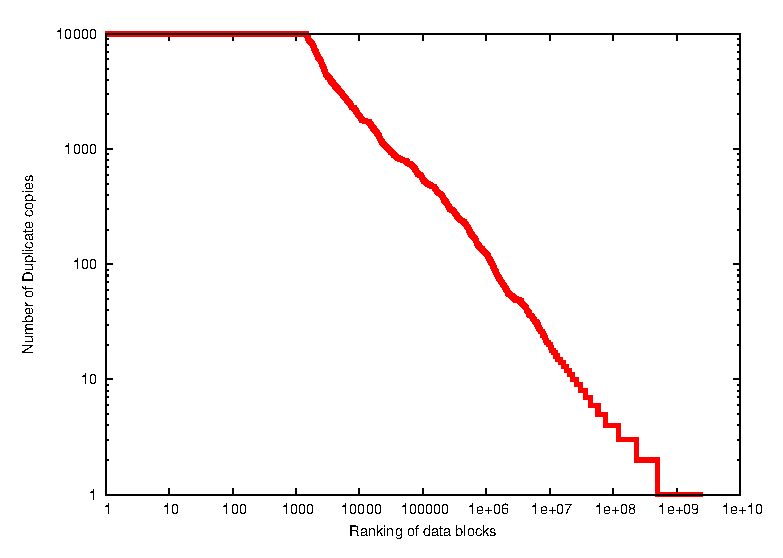
\epsfig{file=images/datadisk.count_rank.eps, width=3in}
\caption{Duplicate count  of common data blocks in a log scale.}
\label{fig:zipf-data}
\end{figure}
Figure \ref{fig:zipf-data} shows the duplicate count  for different data blocks sorted by their ranking in 
terms of the duplication count. $Y$ axis is the popularity of a data block in a log scale 
measured its duplicate count among snapshots. $X$ axis is the identification of data blocks in a log scale
sorted by their duplicate rank.  The rank number  1  is the block with the highest number of duplicates.
The curve exhibits that the popularity of common data blocks partially follows a  Zipf-like distribution.

\begin{figure}
\centering
%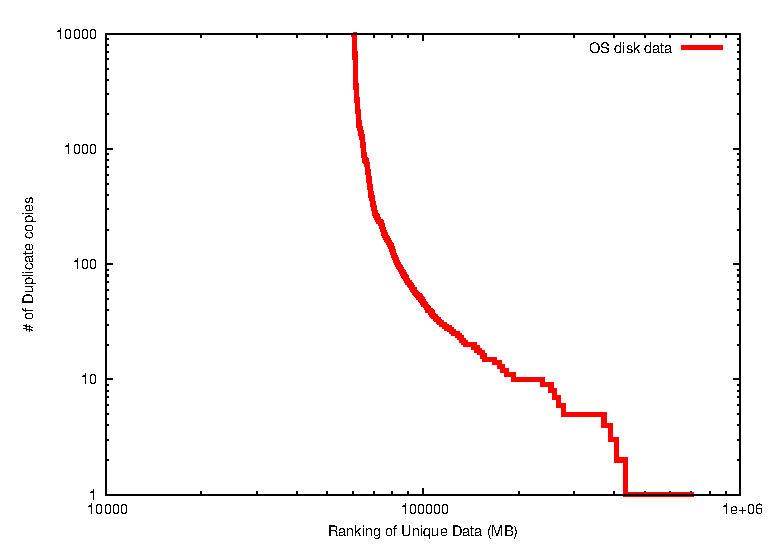
\epsfig{file=images/log-log.35vmos.eps,  width=3in}
%\epsfig{file=images/35os.count_rank.eps, width=3in}
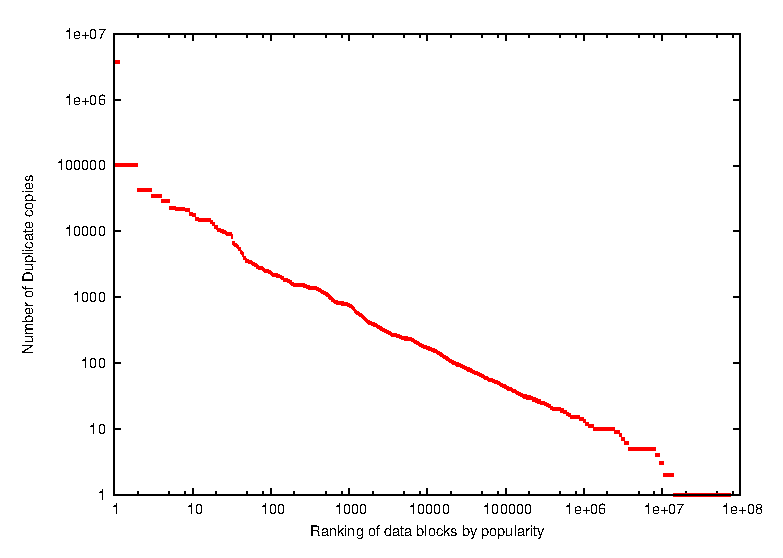
\epsfig{file=images/35vmos.count-rank.eps,width=3in}
\caption{ Duplicate count of  common OS blocks in a log scale.}
\label{fig:OSpopular}
\end{figure}
Figure \ref{fig:OSpopular} shows the duplicate count  for OS disk snapshot blocks sorted by their ranking.
$Y$ axis is the popularity of an OS block in a log scale 
measured its duplicate count among snapshots. $X$ axis is the identification of OS blocks in a log scale
sorted by their duplicate rank.  For the top ranked blocks, there is a flat line in terms of duplicate counts. That
is because there are a large number of OS blocks which have appear in all copies of such OS releases.

}

 
\begin{figure}
\centering
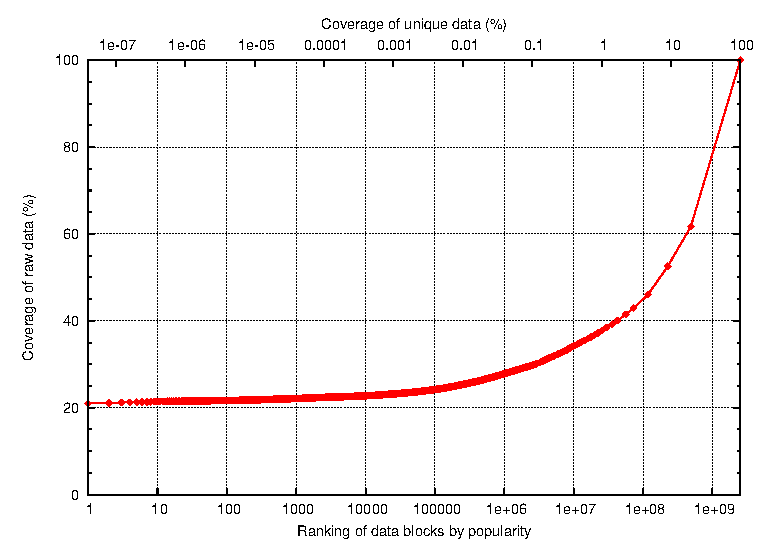
\epsfig{file=images/ay41a_big.data_disk.cdf.eps, width=3in}
%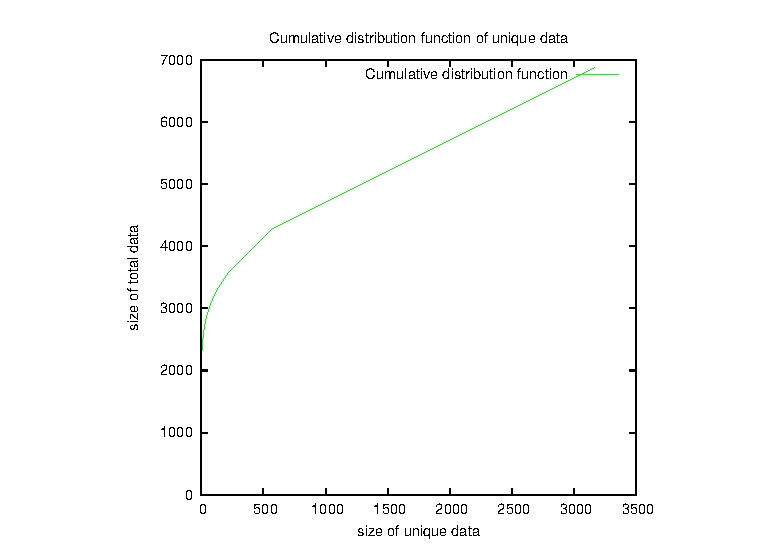
\epsfig{file=images/cdf.disk.v4.eps, width=3in}
%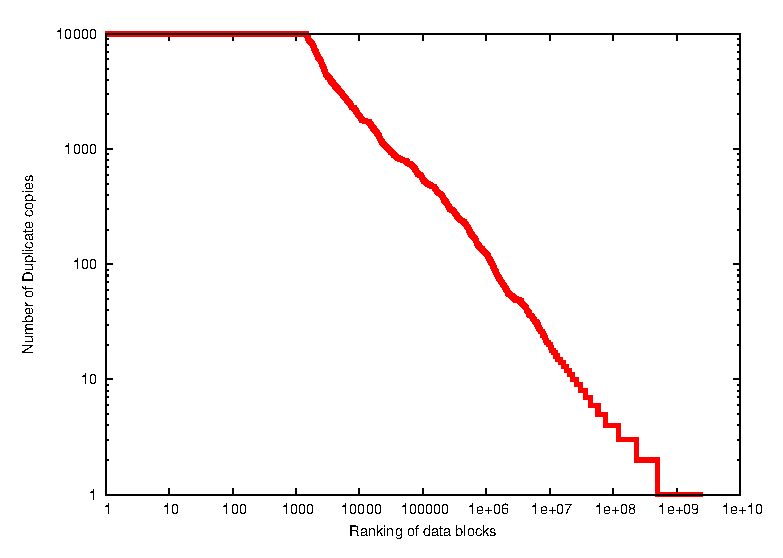
\epsfig{file=images/datadisk.count_rank.eps, width=3in}
%\epsfig{file=images/35os.count_rank.eps, width=3in}

\caption{Cumulative  coverage of popular common user data blocks.}
\label{fig:userdatacoverage}
\end{figure}

We further study how CDS covers content blocks used in image files.
Figure \ref{fig:userdatacoverage} shows the cumulative coverage  ratio of  popular common user data blocks. 
The $X$ axis is the rank of common user data blocks.
Let $S_i$ and $F_I$ be the size and duplicate count 
of the $i$-th block ranked by its duplicate rank.  Then $Y$ axis is the coverage of
the common dataset covering data items from rank 1 to rank $i$. Namely  
\[
\frac{ \sum_{i=1}^{i} S_i * F_i} {\mbox{Total data size}}
\]

Figure~\ref{fig:OSdatacoverage} shows the cumulative coverage  ratio of  popular common OS blocks. 
From both graphs, a small number of most popular common blocks can coverage a large percentage of 
snapshot blocks and thus the size of CDS can be chosen to be small while still having a large
coverage. 
% with $\alpha$ close to 0.78.
%A tiny hottest fraction of data lead to majority of data duplication, as a result, we can target at this small set of commonly seen data
%to design our fast and lightweight deduplication process, just like what people did in CDN and web proxy.

\begin{figure}
\centering
%\epsfig{file=images/cdf.os.v4.eps, width=3in}
%\epsfig{file=images/cdf.os.v4.eps, width=3in}
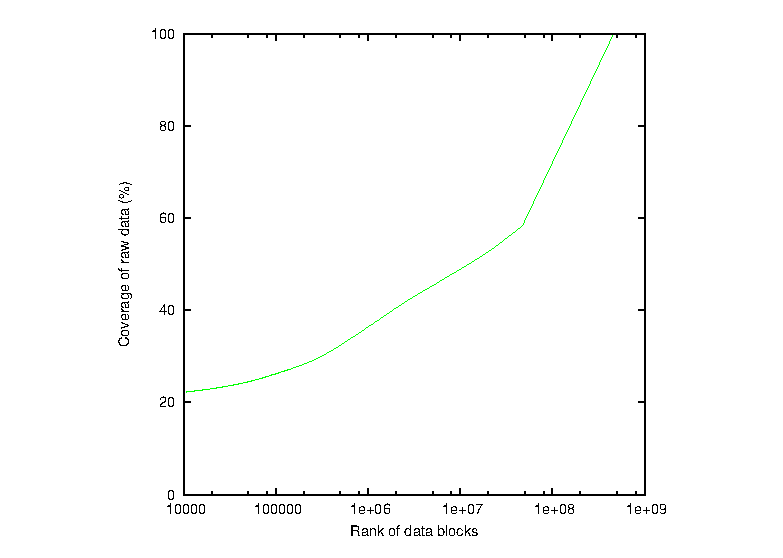
\epsfig{file=images/ay41a_small.os_incremental.cdf.eps, width=3in}
\caption{ Cumulative  coverage of popular common OS disk blocks.}
\label{fig:OSdatacoverage}
\end{figure}


%We define \emph{OS CDS} to be the unchanged data across the base VM image and the snapshots of all
%OS disks which are derived from it. Such data are brought by the operating system and popular 
%software installations, they are rarely modified or deleted, and can be easily extracted using 
%base image data as a hint.



The selection of CDS is completed by separating OS disk and data disk.
While block commonality among data disks may be affected in some degree
 when we scale up the number of total VMs  to be supported,
we expect that  the block commonality among OS disks still remains to be high and  
can be well covered by a fixed CDS because users still adopt common OS releases.
To  verify this,  we examine the percentage of common  OS blocks of the same
release in different VMs  OS releases in Figure~\ref{fig:OSunchanged}. 
%we choose 7 major OSes in Aliyun's
%VM cloud platform and they are: 
%Win2008 Server 64 bits, Win2003 Server 32 bits, Win2003 Server 64 bits, RHEL, CentOS, Ubuntu Server and Debian (all Linux
%distributions are 64 bits).
%we examine 5 VM user disks from each OS, and 10 snapshots for each VM. These VMs have been actively used by their
%owners. Some of  OS disks are modified frequently and in some cases,  users even store a large amount of user data on
%their OS disks. 
%For example, some Ubuntu OS disks have only 2GB of data while some have 50GB.
%For each OS, the base image and all OS
%disk snapshots are divided into variable-sized blocks. Then 
We consider the earlier snapshot for each OS disk as the base image.
For every block in the base image, 
we classify this block as ``completely common''
if  this block has appeared in all snapshots of the same OS release even they are used by different VMs.
Figure \ref{fig:OSunchanged} shows that for each
OS,  at least 70\% of OS blocks are common among all snapshots of the same OS. 
Some latest release  of OS tends to have a higher percentage of content change
while  old release tends to have more variations of content versions.
That can be interpreted as that users with very old  version of operating systems
have a lower tendency to update their OS versions and this causes a larger discrepancy
among OS snapshots of these users.

%into the unchanged category of OS data.

\begin{figure}
\centering
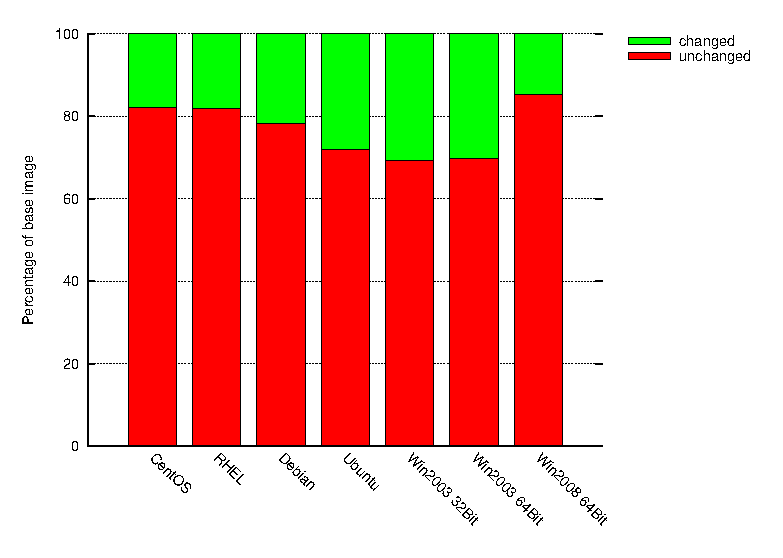
\epsfig{file=images/os_subset.eps, height=2in, width=2.66in}
\caption{Percentage of completely common blocks among different VMs for the same OS release.}
\label{fig:OSunchanged}
\end{figure}

????????????????????????????????????????????????
Based on the above analysis, we have selected a small set of most popular
OS blocks, which is 1.5\% of  unique OS blocks. This set
is quite sufficient to cover the OS related blocks. 
%Then we use this CDS to run the deduplication process again.
That correspond to about  80GB of OS blocks and its corresponding CDS meta occupies 800MB in the cache.
%  data from 350 OS disk snapshots,

%The above analysis is only an estimation of OS and software related common data, 
%some user installed software may not be discovered by this method because they are not 
%included in the base image. However, as we can see in the next section, 
%the overall duplication of user generated data
%follows the Zipf-like distribution, thus all popular data can be discovered by statistic analysis.


%Zipf's law has been shown to characterize use of words in a natural language, city populations, 
%popularity of website visits and other internet traffic data.

%Here we present the first fully consistent empirical study showing that data duplication
%pattern in very large scale storage follows Zipf-like distribution. More specifically,
%we show that the duplication count of any unique data block is inversely proportional to its rank
%in the frequency table, with $\alpha$ smaller than unity. 
%As far as we know, this is the first study of large scale real user data to disclose
%the Zipf-like distribution pattern in data storage area.

%\subsubsection{The model}
%Consider a general storage system that holds user's files without any deduplication. 
%Let $N$ be the total number of unique data blocks after 
%content-defined chunking and deduplication, 
%$C_N(i)$ be the number of duplicate copies that the $i$th data block being
%stored in storage, given all the unique data blocks be ranked in order of their number of duplicate copies.
%Let $S_i$ be the size of $i$th block,
%then the actual ranking of the $i$th block is reflected by $\sum_{1}^{i-1}S_i$. 

%\subsubsection{Methodology}
%1323 users' virtual data disks were scanned using TTTD content-defined chunking, and we performed global perfect deduplication 
%to caculate the number of duplicate copies of each individual unique block. We choose 2KB, 4KB, 16KB as the minimum, average
%and maximum block size, all variable-sized blocks are compared by their SHA-1 hash arther than real data.
%
%We choose user's data disks rather than OS disks in thie experiment for several reasons: First, the data in OS disks are 
%instinctively highly similar, because most of the VM users only make some common or unique but tiny changes to their OSes,
%so the data duplication pattern in OS disks cannot reflect the real distribution of general user data.
%Second, the data disks are way more important in terms of data safty and backup because they are 
%what users really care about.

\comments{
\subsection{Discussion}
By storing the hash index of a small set of hottest data (CDS), we expect to achieve great 
deduplication effect with minimal cost.
But one problem of the CDS is what we called \emph{blind spot}: the update of CDS is always 
behind new data's arrival,
as a result, some data must have been written to the backup store before being collected into CDS, thus such 
duplication may comprise the effect of
CDS. For instance, when a MySQL update is released, some users may apply it very quickly, so the new hot data bring by
this update will not be filtered by CDS. Only until later our CDS update includes those new data, then the rest of MySQL users get benefited.
We can take a few measurements to reduce the impact of blind spot. First, the data in blind spot will not accumulate, because snapshots backup
is a paid service, so over the long term, data in blind spot will be removed from backup store as VMs and old snapshots keep being deleted.
Second, for the major OS updates, we can anticipate them in advance by putting the new hot data into CDS before users widely adopt them.

Another problem associated with CDS is that some data in CDS may no longer be popular or even disappear
as time goes. For example, an MySQL software update may invalidate some data that we previously hold in 
the CDS. If some data blocks in CDS are no longer referenced, our map-reduce process is able to detect
this situation, so invalid data will be removed and new data will be added during the next CDS update. 
But if some users choose to keep their old MySQL version, then the corresponding old and new data will co-exist in the CDS.
}



%In our snapshot deduplication architecture, CDS is the key to achieve greater deduplication than
%incremental backup solutions. Our basic assumption of CDS us that VM disks, especially OS disks,
%have huge amount of data in common, and such common data can be represented by a relatively smaller data set
%because of their high appearence frequency. As a result, the major portion of snapshot deduplication effect shall 
%emerge from eliminating the duplication of such a small data set. In this section, we evaluate
%the effectiveness of CDS using real user VM disks from our production VM cluster.


\subsection{A comparison of perfect and CDS-based deduplication }
%Figure~\ref{fig:pd} shows the compression ratio of perfect deduplication at different dataset sizes
%as we vary the data size from about 4 terabytes to about 23.5 terabytes.
After level-1 and level 2 elimination, our experiment shows that 
the full deduplication would reduce the storage  further   by  45\% to 53\% of user disk space. 
If we put all these unique data into CDS, we could achieve full deduplication,
but the CDS size is not affordable. So we evaluate how much space saving of 
deduplication can be achieved when varying the CDS size.
%\begin{figure}
%  \centering
%  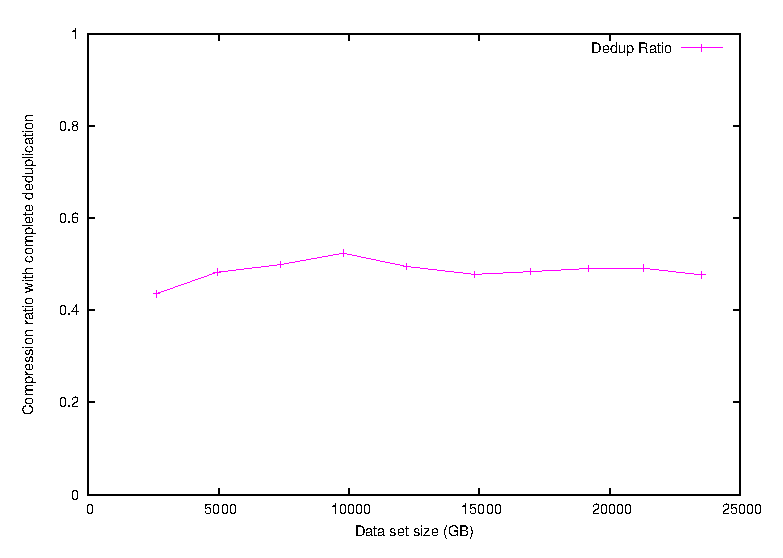
\epsfig{file=images/dedup_ratio.eps, height=2in, width=2.66in}
%  \caption{Perfect deduplication on data disks}
%  \label{fig:pd}
%\end{figure}

%We rank unique data blocks by their duplication count, and choose the hottest blocks as CDS. 
Figure \ref{fig:datacdssize} shows the relationship between CDS cache size and relative space saving ratio
compared to the full deduplication.  The unit of CDS size is gigabytes.
We define \emph{space saving ratio} as the space saving of the CDS method divided by 
full deduplication saving ratio. 
With a small amount of CDS data can still  accomplish more than 50\% of what perfect deduplication can do.
%But this effect decreases when more data are added to CDS. 
%The lower bound of CDS space saving ratio is 50\%, which is very easy to accomplish. 

\begin{figure}
  \centering
  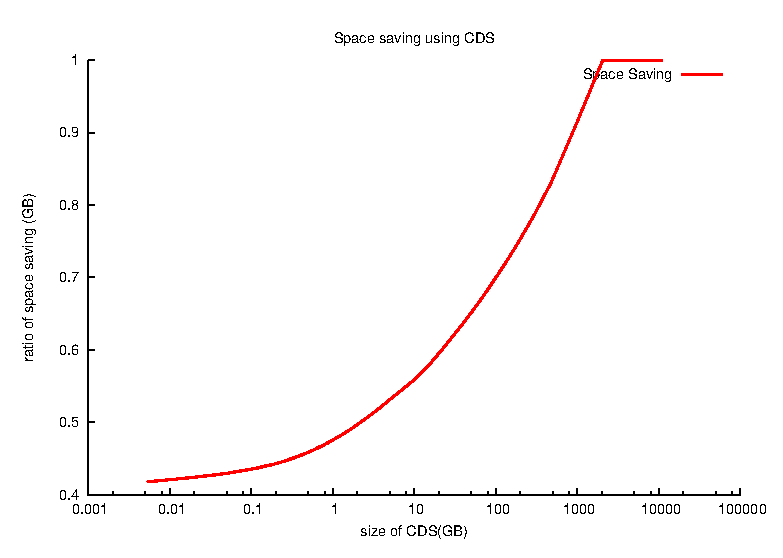
\epsfig{file=images/uniquedata-saving.eps, width=3in}
  \caption{Relative ratio of space size compared to full deduplication when CDS size changes.}
  \label{fig:datacdssize}
\end{figure}

CDS size is restricted by system memory resource.
Figure \ref{fig:datacds} shows how CDS space saving is affected by the system scale in terms of
the dataset size. 
In this experiment we first set out a goal of space saving ratio, 
then watch how much data needs to be placed in CDS cache to achieve this goal.
From the graph we can see a 75\% saving goal lead to a stable ratio between 
CDS size and data size, which requires 0.01\% of data to be put in CDS.

Base on above data we can estimate the size of data CDS and its effect. 
Currently we prepared 500MB memory per machine to store CDS meta, then it can represent 50GB of data. 
If we assume each VM has 30GB of user data at runtime, and we host 25 VMs per machine, 
 maintain 10 snapshots per VM, each brings 10\% additional modified data. 
Thus the user data in snapshot system is 1.5TB per machine. So the upper bound of 
$CDS size/ Data size = 0.033$, which is sufficient for the 75\% saving goal.

\begin{figure}
  \centering
  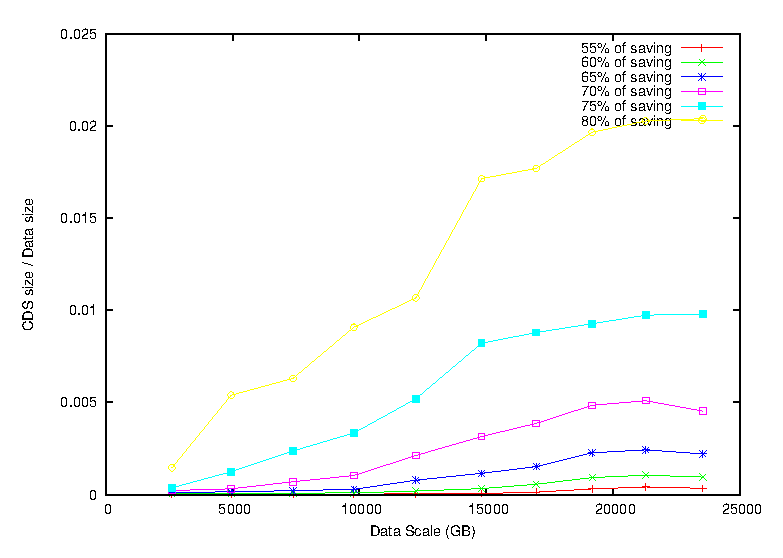
\epsfig{file=images/cds_scale.0.7.eps, width=3in}
  \caption{The relative size ratio of  CDS over the data size. }
  \label{fig:datacds}
\end{figure}

%Unlike the CDS of OS disks which is mainly composed of OS related data thus highly predictable, 
%data disks is unpredictable because we cannot control what user can put in there. But we still
%suspect that highly duplicated data in existing data are very likely to be duplicated again.
%So we randomly pick 50 out of 1322 data disks as the new data, and use the rest as existing data
%to extract CDS. Using 1.5\% as CDS threshold, we see the total 1198GB of new data is reduced by 
%755.8GB, while perfect deduplication can reduce 1017.4GB. So 74.3\% of duplicate blocks are eliminated 
%by pre-trained CDS, which is quite satisfactory.
 %data study, zipf, model of cds size and dedup efficiency
%\section{Results}
In our snapshot deduplication architecture, CDS is the key to achieve greater deduplication than
incremental backup solutions. Our basic assumption of CDS us that VM disks, especially OS disks,
have huge amount of data in common, and such common data can be represented by a relatively smaller data set
because of their high appearence frequency. As a result, the major portion of snapshot deduplication effect shall 
emerge from eliminating the duplication of such a small data set. In this section, we evaluate
the effectiveness of CDS using real user VM disks from our production VM cluster.

\subsection{Experiment Setup}
The data set we use is the same as described in previous section. 
We choose extreme binning and perfect deduplication to compare against.
In all experiments, our deduplication enforces 2MB fix-sized segment boundary, 
and uses TTTD algorithm to divide segment into 4KB variable-sized blocks.
For perfect deduplication and extreme binning, the whole snapshots are splitted
using TTTD with 4KB average size. The original extreme binning paper uses whole file
as the input unit, but that is way too big for our system. 
Thus we split image snapshot files into variable-sized segments base on the block hash list, 
using TTTD with average size of 2MB.

\subsection{OS Disk}
We extract the CDS of OS disks by counting the blocks that will appear in a VM's
block store if no CDS is involved in the deduplication process. The threshold is set to less than
1.5\%, which is quite sufficient to include the OS related data since their duplication is much
heavier than others. Then we use this CDS to run the deduplication process again.
Finally we extracted about 80GB of CDS data from 350 OS disk snapshots,
the corresponding CDS meta occupies 800MB in CDS cache.

\begin{figure}
  \centering
  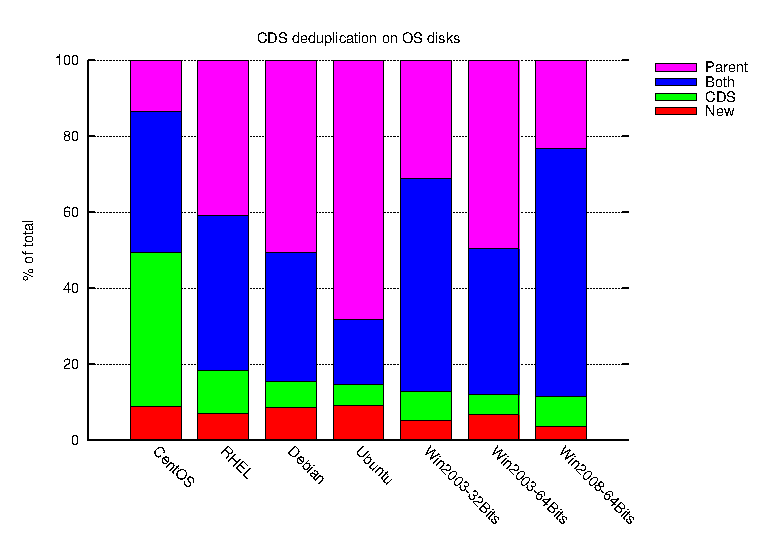
\epsfig{file=images/os_cds_sim.eps, height=2in, width=2.66in}
  \caption{CDS deduplication effect on OS disks}
  \label{fig:oscds}
\end{figure}

For each block, we tag it with one of the following:
\begin{itemize}
\item {New: this block cannot be deduplicated and thus write to block store.}
\item {CDS: this block is deduplicated by CDS.}
\item {Parent: this block is not found in CDS, but is found in parent snapshot's segment recipe.}
\item {Both: this block is both found in CDS and parent snapshot.}
\end{itemize}
As we can see from \ref{fig:oscds}, locality dominates.
This is because the interval between two snapshots is quite short due to our daily snapshot strategy. 
However, locality still doesn't work well on some of the OSes. But CDS, on the contrary,
finds a lot of duplicates that locality can't find, especially in a VM's first snapshot.

Combining all the VMs, we see the overall 7.4TB of data is reduced to 512GB. Extreme bining 
reduces this data set to 542GB, which is slightly worse. As a reference, perfect deduplication achieves
364GB in this experiment.

Overall, none of locality or CDS can solely work well, but by combining them together 
we get fairly good and stable deduplication ratio to all kind of OSes. If compare to all
incremental backup solutions, CDS can save addition 50\%+ of disk space because it greatly reduces
the cross-VM duplicates.

\subsection{Data Disk}
Figure \ref{fig:pd} shows the compression ratio of perfect deduplication at different data scales. 
Basically perfect deduplication would help us save 50\% of space on user data, 
regardless of scale. If we put all these unique data into CDS, we could achieve perfect deduplication, 
which is not affordable. So we need to see how much space saving of perfect 
deduplication can be achieved through a limit size CDS.
\begin{figure}
  \centering
  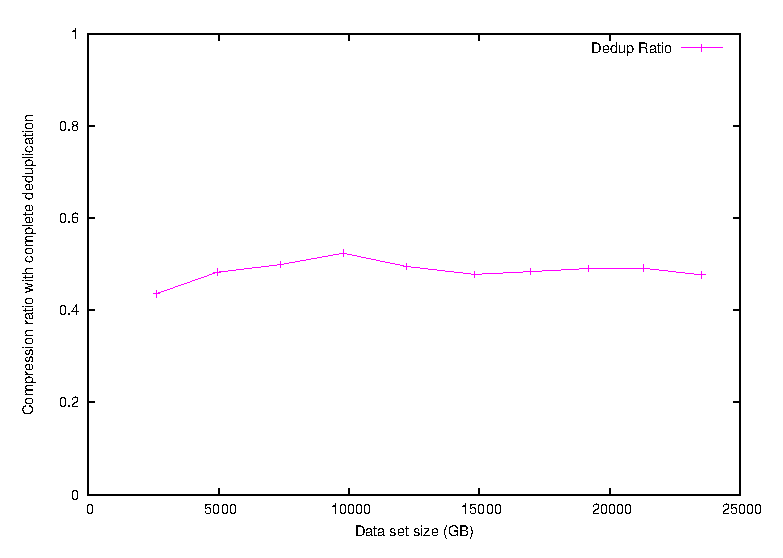
\epsfig{file=images/dedup_ratio.eps, height=2in, width=2.66in}
  \caption{Perfect deduplication on data disks}
  \label{fig:pd}
\end{figure}

We rank unique data blocks by their duplication count, 
and choose the hottest blocks as CDS. 
We define \emph{space saving ratio} as the space saving of CDS divide by 
perfect deduplication saving. Figure \ref{fig:datacdssize} shows the relationship between CDS size and space saving. 
It’s clear a very small amount of CDS data provides more than 50\% saving. 
But this effect decreases when more data are added to CDS. 
The lower bound of CDS space saving ratio is 50\%, which is very easy to accomplish. 

\begin{figure}
  \centering
  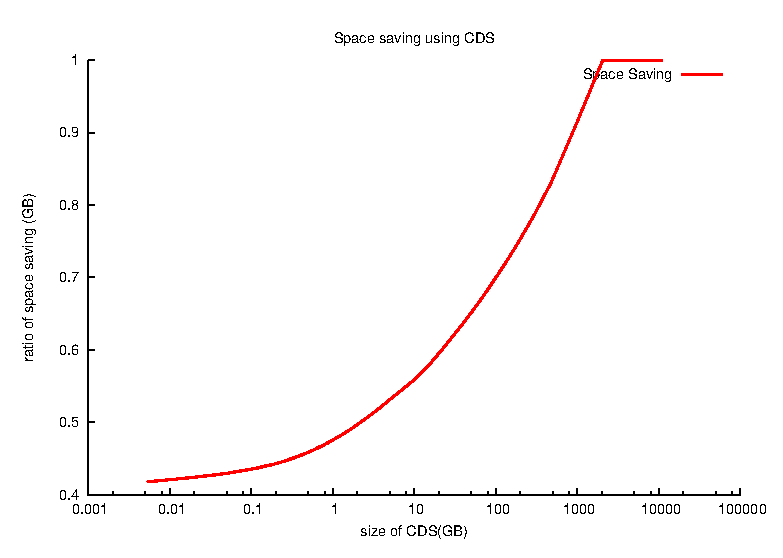
\epsfig{file=images/uniquedata-saving.eps, height=2in, width=2.66in}
  \caption{Size of CDS vesus space saving}
  \label{fig:datacdssize}
\end{figure}

The upper bound of CDS size is restricted by system memory resource.
Figure \ref{fig:datacds} shows how CDS space saving is affected by the system scale. 
In this experiment we first set out a goal of space saving ratio, 
then we watch how much data we need to put into CDS to achieve this goal.
From the graph we can see a 75\% saving goal lead to a stable ratio between 
CDS size and data size, which requires 0.01\% of data to be put in CDS.

Base on above data we can estimate the size of data CDS and its effect. 
Currently we prepared 500MB memory per machine to store CDS meta, then it can represent 50GB of data. 
If we assume each VM has 30GB of user data at runtime, and we host 25 VMs per machine, 
 maintain 10 snapshots per VM, each brings 10\% additional modified data. 
Thus the user data in snapshot system is 1.5TB per machine. So the upper bound of 
$CDS size/ Data size = 0.033$, which is sufficient for the 75\% saving goal.

\begin{figure}
  \centering
  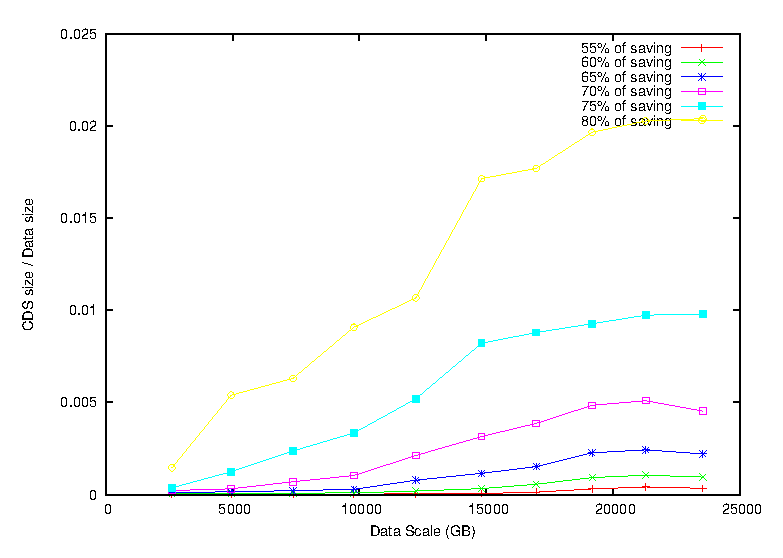
\epsfig{file=images/cds_scale.0.7.eps, height=2in, width=2.66in}
  \caption{CDS deduplication effect on data disks}
  \label{fig:datacds}
\end{figure}

Unlike the CDS of OS disks which is mainly composed of OS related data thus highly predictable, 
data disks is unpredictable because we cannot control what user can put in there. But we still
suspect that highly duplicated data in existing data are very likely to be duplicated again.
So we randomly pick 50 out of 1322 data disks as the new data, and use the rest as existing data
to extract CDS. Using 1.5\% as CDS threshold, we see the total 1198GB of new data is reduced by 
755.8GB, while perfect deduplication can reduce 1017.4GB. So 74.3\% of duplicate blocks are eliminated 
by pre-trained CDS, which is quite satisfiable.

%\section{Related Works}
Several approaches have been previously proposed to enable efficient deduplication in D2D backup.

DDFS\cite{bottleneck08} exploits chunk locality to achieve high-throughput perfect deduplication. 
It preserves locality by a Stream-Informed Segment Layout and exploits locality with Locality Preserved Cache. 
An in-memory Bloom Filter is also used to accelerate non-duplicate chunk identification.

Sparse Indexing\cite{sparseindex09} is an approximate deduplication technique designed for D2D backup. 
It divides data stream into variable-sized multiple kilobytes chunks, and construct multiple megabytes segments
using the same chunking technique, 
which are then sampled and mapped to a compact in-memory sparse index. 
Incoming segments are only deduplicated against several existing similar 
segments selected according to the sparse index.

Both DDFS and Sparse Indexing are designed for D2D backup workloads, 
and do not address the scalability issue in a distributed environment. 
A few scalable deduplication approaches have been proposed recently.

Extreme Binning\cite{extreme_binning09} is a scalable parallel deduplication approach 
that targets at non-traditional backup workloads that consist of low-locality individual files. 
It groups highly similar files into bins, and eliminates duplicate chunks inside each bin. 
Duplicate chunks are allowed to exist among different bins, resulting in approximate deduplication. 
By keeping only the primary index in memory, Extreme Binning can reduce the RAM requirement while 
maintaining a reasonably high throughput. However, their per-file based similarity detection 
is going to group all similar files into one node, which will break load balancing if some files are
huge and similar(e.g., virtual machine images).

MAD2\cite{mad210} is a scalable high-throughput exact duplication approach. 
MAD2 utilizes on-disk Hash Bucket Matrix to preserve fingerprint locality and 
integrates in-memory Dual Cache to capture and exploit locality. 
In addition, MAD2 employs Bloom Filter Array to efficiently identify unique 
incoming fingerprints and indicate where a duplicate may reside. 
By employing a DHT-based Load-Balance technique to distribute file recipes 
and chunk contents among multiple storage nodes in their backup sequences, 
MAD2 further enhances performance with a well balanced load. However, the
data locality does not exist for cloud storage because only changed chunks are expected
to be uploaded, and
the heavy usage of memory and CPU indicates such exact deduplication backup systems
need storage-exclusive servers with hardware replication support, which is not a general case 
for the cloud..

HYDRAstor\cite{hydrastor09}, a scalable secondary storage solution, 
constructs its backend using a grid of storage nodes built around a distributed hash table. 
The backend maintains large-scale variable-sized, content-addressed, immutable, 
and highly-resilient data blocks that are logically organized in a directed acyclic graph. 
Duplicate chunks are eliminated according to their hashes. 
HYDRAstor adopts an average chunk size of 64KB, among other constraints, 
to keep all the metadata in memory and avoid the duplicate-lookup disk bottleneck. 
This degrades the space efficiency of deduplication, and still requires huge amount of memory.

We believe a deduplication backend of cloud storage must have scalability and
 high availability built in mind, being able to run on low-cost non-proprietary machines.
  Unlike sloud, all above systems lack one or a few such properties. All exact deduplication approaches
are too costly, this is why we choose similarity based approach to trade deduplication
accuracy for speed. 

Eariler deduplication systems mainly focus on improving storage space efficiency by eliminating 
duplicates at the file level, fixed-size block level, or variable-sized chunk level. 
EMC's Centera\cite{emc_centera} identify and eliminate duplicate data by comparing 
the hash of the whole file or fixed content. Venti\cite{venti02}, a block-level archival storage, 
removes redundant fixed-size data blocks by comparing their secure hashes. Pastiche\cite{pastiche02} 
utilizes chunk-level duplicate detection to construct a resource-saving peer-to-peer backup network. 
Deep Store\cite{deepstore05}, a large scale archival storage system, uses both variable-sized 
chunk-level deduplication and delta compression to save storage. Jumbo Store\cite{jumbo07} organizes 
variable-sized chunks into Hash-Based Directed Acyclic Graphs to save both storage and 
bandwidth while performing incremental upload and versioning for a utility rendering service. 

Duplicate detection technique has also been used in bandwidth-saving synchronization protocols\cite{rsync} 
and low-bandwidth network file systems\cite{lbfs01}.
%\input{future}
\section{Conclusion}
\label{sect:final}
The main contribution of this paper is a multi-level selective deduplication scheme among VM snapshots. 
Inner-VM deduplication localizes backup data dependence and exposes more parallelism  
while global deduplication using a small common data set appeared in OS and data disks
effectively  covers a large amount of snapshot blocks.
Our evaluation using Aliyun's data has shown that 
level 1 and level 2 deduplication can reduce the storage need by 78\% while level 2 inner 
fingerprint comparsion contributes 4.5\%%. 
Level 3 can add additional 10.5\% reduction and accomplish 75\% of what full fingerprint-based
deduplication can do. Our scheme uses a very small amount of memory on each node, and leaves
room for additional optimization we are further studying.
%Noted that 6\% is still significant, which is about 24GB per each VM and for a 1000 node Aliyun cluster,
%this is about 600 terabytes.
 
%Our experiments show th
%our solution can eliminate the majority of data duplication with a tiny fraction of
%block hash index store in memory. It does not only saves valuable system resouces in
%the VM cloud, but also makes deduplication much faster.
%
%
%Using  50 user VM data out of 1322 data disks as the training data and
%with  1.5\% as CDS threshold, we see the total 1198GB of new data is reduced by
%755.8GB, while perfect deduplication can reduce 1017.4GB. So 74.3\% of duplicate blocks are eliminated
%by pre-trained CDS, which is quite satisfactory.



      %\setlength{\itemsep}{ex}%
%      \setlength{\parskip}{0ex}%
%\setlength{\itemsep}{-3mm}

	%\linespread{0.3} 
  \let\oldthebibliography=\thebibliography
  \let\endoldthebibliography=\endthebibliography
  \renewenvironment{thebibliography}[1]{%
    \begin{oldthebibliography}{#1}%
      \setlength{\parskip}{-0.02ex}%
      \setlength{\itemsep}{-0.02ex}%
      \setlength{\baselineskip}{-0.02ex}%

  }%
  {%
    \end{oldthebibliography}%
  }
{\small
\bibliographystyle{abbrv}
\bibliography{dedup,dedup1}
}
\end{document}
